\documentclass{beamer}
\usepackage{tipa}
\usepackage{phonrule}
%\setbeamersize{text margin left=10pt,text margin right=10pt}
\usetheme[numbering=none]{metropolis}
\usepackage{media9}
\usepackage{listings}
\usepackage{amsfonts}
\usepackage{dsfont}
\usepackage{amsmath}
\usepackage{bbm}
\usepackage{verbatim}
\usepackage{phonrule}
%\usepackage{tipa}
\usepackage{tikz}
\usetikzlibrary{fit}
\usepackage{color}
\usepackage{booktabs}
\usepackage{tipa}
\usepackage{amssymb}
\usepackage{verbatim}
\usepackage[absolute,overlay]{textpos}
\usepackage{pifont}% http://ctan.org/pkg/pifont
\usepackage{caption}
\usepackage{subcaption}
\newcommand{\cmark}{\ding{51}}%
\newcommand{\xmark}{\ding{55}}%
\usetikzlibrary{bayesnet}
\usetikzlibrary{decorations.markings}
\usetikzlibrary{decorations.pathmorphing}
\tikzset{squiggle/.style={decorate, decoration={snake,amplitude=.4mm}}}
\usepackage{xcolor}
\definecolor{pop1}{HTML}{1F78b4}
\definecolor{pop2}{HTML}{164C13}
\definecolor{pop3}{HTML}{d95F02}
\definecolor{orange}{HTML}{d95F02}
\definecolor{teal}{HTML}{1b9e77}
\newcommand{\pop}[1]{\textcolor{pop1}{#1}}
\newcommand{\popp}[1]{\textcolor{pop2}{#1}}
\newcommand{\tree}[1]{\textcolor{pop3}{#1}}
\newcommand{\orange}[1]{\textcolor{orange}{#1}}
\newcommand{\teal}[1]{\textcolor{teal}{#1}}
\newcommand{\code}[1]{{\footnotesize\texttt{#1}}}
\newcommand{\greenCode}[1]{{\footnotesize\popp{\code{#1}}}}
\newcommand{\blueCode}[1]{{\footnotesize\pop{\code{#1}}}}
\definecolor{backgroundGreen}{HTML}{23373b}
\lstset{escapeinside={<@}{@>}}
\usepackage{pgf}  

%% \usepackage[sfdefault]{FiraSans} %% option 'sfdefault' activates Fira Sans as the default text font
%% \usepackage[T1]{fontenc}
%% \renewcommand*\oldstylenums[1]{{\firaoldstyle #1}}

\newcommand{\closex}[2]{
  \renewcommand{\arraystretch}{#1}
  #2
  \renewcommand{\arraystretch}{1}
}
\newcommand{\closey}[2]{
  \setlength{\tabcolsep}{#1}
  #2
  \setlength{\tabcolsep}{6pt}
}

\newcommand{\person}[2]{\closex{0.2}{\begin{tabular}{c}
    {\footnotesize #1}\\
    \includegraphics[width = 1.7cm]{#2}
\end{tabular}}}
\newcommand{\bigPerson}[2]{\closex{0.2}{\begin{tabular}{c}
    {#1}\\
    \includegraphics[width = 3cm]{#2}
\end{tabular}}}


\newcommand{\Expect}{\mathds{E}} %{{\rm I\kern-.3em E}}
\newcommand{\indicator}{\mathds{1}} %{{\rm I\kern-.3em E}}
\newcommand{\expect}{\mathds{E}} %{{\rm I\kern-.3em E}}
\newcommand{\probability}{\mathds{P}} %{{\rm I\kern-.3em P}}
\DeclareMathOperator*{\argmin}{arg\,min} % thin space, limits underneath in displays
\DeclareMathOperator*{\argmax}{arg\,max} % thin space, limits underneath in displays

\usepackage[absolute,overlay]{textpos}

\newcommand{\nextForm}[1]{\rotatebox[origin=c]{270}{$_{\curvearrowright}$}$_{#1}$}
 
\usepackage{amsfonts}
\usepackage{tabularx}
%\usepackage{color}
\usepackage{graphicx}
\usepackage{booktabs}
\usepackage{xcolor}
\usepackage{tikz}
\usetikzlibrary{trees}
\usetikzlibrary{fit}
\usetikzlibrary{calc}
\usetikzlibrary{bayesnet}
\usepackage[absolute,overlay]{textpos}
\usepackage{stmaryrd}
\newcommand{\sem}[1]{\llbracket #1\rrbracket}
\newcommand{\tuple}[1]{\ensuremath{\left \langle #1\right \rangle}}
\newcommand{\messageOverlay}[1]{
      \tikz[overlay,remember picture]
      \node[align=left,fill=backgroundGreen,text=white] at (current page.center){#1};
}
\newcommand{\myPaper}[1]{
  \tikz[overlay,remember picture]
  \node[anchor=south west,align=left] at (current page.south west){#1};
}
\newcommand{\myPaperRight}[1]{
  \tikz[overlay,remember picture]
  \node[anchor=south east,align=left] at (current page.south east){#1};
}
\usepackage{booktabs}
\usepackage{tipa}
\usepackage{amssymb}
\usepackage{verbatim}
\usepackage[absolute,overlay]{textpos}
\usepackage{pifont}% http://ctan.org/pkg/pifont
%% \newcommand{\cmark}{\ding{51}}%
%% \newcommand{\xmark}{\ding{55}}%
\usetikzlibrary{bayesnet}
\usetikzlibrary{decorations.markings}

\newcommand\Wider[2][3em]{%
\makebox[\linewidth][c]{%
  \begin{minipage}{\dimexpr\textwidth+#1\relax}
  \raggedright#2
  \end{minipage}%
  }%
}
\definecolor{backgroundBeige}{RGB}{250,250,250}
\newcommand{\denotation}[1]{{\llbracket #1 \rrbracket}}

\usepackage[utf8]{inputenc}
\newcommand{\reduce}{\longrightarrow}
\usepackage{amssymb}% http://ctan.org/pkg/amssymb
\usepackage{pifont}% http://ctan.org/pkg/pifont

\usepackage{fancyvrb}

\usepackage[most]{tcolorbox}
\definecolor{block-gray}{gray}{0.10}
\newtcolorbox{mycode}{colback=block-gray,grow to right by=0mm,grow to left
by=0mm, boxrule=0pt,boxsep=0pt,breakable,fontupper=\color{white}}

%% Program ::=
%%   (if Bool List
%%     (append RecursiveList
%%             RecursiveList
%%             RecursiveList))
%% RecursiveList ::= List
%%          | (recurse List)

            

\usepackage{arydshln}

%\newcommand{\Expect}{\mathds{E}} %{{\rm I\kern-.3em E}}
\newcommand{\Probability}{\mathds{P}} %{{\rm I\kern-.3em P}}
%\usepackage{cancel}
%\DeclareMathOperator*{\argmax}{arg\,max}
%Information to be included in the title page:
%\usepackage{soul}
\usepackage[normalem]{ulem}
\title{The Role of Higher-level Knowledge\\in Discovery Problems:\\Programs and Hierarchical Bayes}
\author{Kevin Ellis}
\institute{Cornell} 
\date{2021 Workshop on Artificial Scientific Discovery}
  
 
\begin{document}
 
\frame{\titlepage}

\begin{frame}{}

  1. Scientific models\visible<2->{ as \textbf{generative programs}}
  

  2. Discovery\visible<3->{ as \textbf{program synthesis}}

  3. Higher-level knowledge\visible<4->{ as \textbf{Bayesian prior} over programs}

\end{frame}

\begin{frame}{}
  \Wider[3em]{
    \only<1>{\includegraphics[width = \textwidth]{tu6}}
    \only<2>{\includegraphics[width = \textwidth]{tu5}}
    \only<3>{\includegraphics[width = \textwidth]{tu4}}
    \only<4>{\includegraphics[width = \textwidth]{tu3}}
    \only<5>{\includegraphics[width = \textwidth]{tu2}}
    \only<6>{\includegraphics[width = \textwidth]{tu1}}
    \only<7>{\includegraphics[width = \textwidth]{tu}}
  }

  \end{frame}

\begin{frame}{Why programs?}
  \Wider[6.5em]{  \begin{tabular}{ccc}
    \visible<2->{\begin{tabular}{l}
      strong generalization\\
    \end{tabular}}&
    \visible<3->{\begin{tabular}{l}
      interpretability\\
    \end{tabular}}
    &\visible<4->{\begin{tabular}{l}
       universal expressivity\\
     \end{tabular}}\\
    \visible<2->{
      \begin{tabular}{c}
        \includegraphics[width = 3cm]{figures/polynomialExtrapolation}\\
        {\small\texttt{f(x)=(x-1)**2 - 0.5}}
    \end{tabular}}&
    \visible<3->{\begin{tabular}{c}
        \includegraphics[width = 3.5cm]{figures/explodedCAD}\\\emph{vs}\\
        \includegraphics[width = 3.5cm]{figures/drillMesh}
    \end{tabular}}&
    \visible<4->{%% \includegraphics[width = 4cm]{figures/turingMachine}
      \begin{tabular}{c}
        \includegraphics[width = 3cm]{figures/famous}
    \end{tabular}}
  \end{tabular}}

  \visible<5->{\messageOverlay{\large main challenge:\\\large combinatorial search}}

\end{frame}



\begin{frame}{}
  \begin{center}
    \begin{tabular}{l}
      {\textcolor{black}{Higher-level Knowledge: Case study in linguistics}}\\
      {\textcolor{black}{Higher-level Knowledge: General program discovery}}
      \end{tabular}
  \end{center}
\end{frame}
\begin{frame}{}
  \begin{center}
    \begin{tabular}{l}
      {\textcolor{black}{Higher-level Knowledge: Case study in linguistics}}\\
      {\textcolor{gray}{Higher-level Knowledge: General program discovery}}
      \end{tabular}
  \end{center}
\end{frame}

\begin{frame}[fragile]{Scientific discovery}

  \Wider[4em]{
    \includegraphics[width = 0.8\textwidth]{figures/distillingLaws}\\
                    {\small Schmidt \& Lipson: ``Distilling Free-Form Natural Laws from Experimental Data''}

                    \\\vspace{1cm}\\
                    \begin{tabular}{cc}
                      \begin{tabular}{c}
                        \includegraphics[width = 0.45\textwidth]{figures/genetics}
                        \end{tabular}&
                      %% \visible<2>{\hspace*{-0.5cm}\includegraphics[width = 0.53\textwidth]{figures/solomonScience2}}\\
                      \begin{tabular}{l}
                        {\small Lezon et al. 2006}\\{\small inferring genetic interaction networks}
                      \end{tabular}&
                      \end{tabular}
  }

\end{frame}

\begin{frame}[fragile]{Discovering human-understandable models of language}
  \begin{center}
    \begin{tikzpicture}[scale=0.75]
      \input{phonology/languageWheel50.tex}
    \end{tikzpicture}
  \end{center}
%%   \pause
%%   \messageOverlay{\large many languages, 70 diverse benchmarks\\\\
%%     \large linguists distill out higher-level knowledge: ``universal grammar''\\\\
%% \large children and linguists can learn from sparse data\\\\
  %% \large  linguists can communicate their knowledge}
  \begin{tikzpicture}[remember picture, overlay,label distance=-2mm] \node[anchor=south east, label={Tim O'Donnell}] at (current page.south east) {\includegraphics[width = 2cm]{collaborators/Timothy}}; \end{tikzpicture}
\end{frame}

\begin{frame}{Few-shot language learning experiment}
  Mandarin:

  \vspace{1cm}

  \begin{tabular}{rcc}
    & adjective & adverb\\
    ``slow'' & \textipa{man} & \textipa{manmand@}\\
    ``small'' & \textipa{xiao} & \textipa{xiaoxiaod@}\\
    ``fast'' & \textipa{kuai} & \only<2->{\textipa{kuaikuaid@}}\only<1>{???}
  \end{tabular}

  \vspace{1cm}
  
  \only<3>{stem+stem+\textipa{d@}}

  \end{frame}

\begin{frame}{Few-shot language learning experiment}
  Serbo-Croatian:
  \vspace{1cm}
  
  \begin{tabular}{rlll}
    &\multicolumn{1}{c}{masculine}&\multicolumn{1}{c}{feminine}&%% \only<5->{stem (unobserved)}
    \\
    ``rich''&\textipa{bogat}&\textipa{bogata}&%% \only<5->{bogat}
    \\
    ``mild''&\textipa{blag}&\textipa{blaga}&%% \only<5->{blag}
    \\
    ``green''&\textipa{zelen}&\only<1>{???}\only<2->{\textipa{zelena}}&%% \only<5->{zelen}
    \\
    \only<4->{``clear''}&\only<4>{???}\only<5>{\textbf{yasan}}& \only<4->{yasna}&%% \only<5->{yasn}
    \\  
  \end{tabular}

  \vspace{1cm}
  
  \only<3->{\emph{add ``a'' to stem to make feminine}}
  
  \only<5->{
    \emph{insert ``a'' between two word-final consonants}\\
    \phonb{$\varnothing$}{a}{C}{C\#}
  }

\end{frame}


%% \begin{frame}{Diverse Linguistic Phenomena}
%%   \includegraphics[width = \textwidth]{phonology/Croatian}
%% \end{frame}
%% \begin{frame}{Languages with tones}
%%   \includegraphics[width = \textwidth]{phonology/tonal}
%% \end{frame}
\begin{frame}
  \begin{center}
    \begin{tabular}{ccc}
      \includegraphics[width = 0.3\textwidth]{figures/odden}&
      \includegraphics[width = 0.3\textwidth]{figures/spe}&
      \includegraphics[width = 0.3\textwidth]{figures/roca}
    \end{tabular}
  \end{center}
\end{frame}
\begin{frame}{}
\Wider[5em]{  \includegraphics[width = \textwidth]{figures/Turkish1}}
\end{frame}
\begin{frame}{Turkic Sakha (Yakut)}
  \newcommand{\R}[1]{$\xrightarrow{r_{#1}}$}
\newcommand{\li}[2]{$\text{\textsc{#2}}: \text{\textipa{#1}}$}

\usetikzlibrary{calc}

\definecolor{observationColor}{RGB}{204,51,0}
\definecolor{languageColor}{RGB}{0,128,102}
\definecolor{lexiconColor}{RGB}{51,76,128}
\definecolor{universalColor}{RGB}{255,128,128}

\newcommand{\surfaceTriple}[4]{\phantom{t}\textcolor{observationColor}{\textsc{#1}}&\surface{#2}&\surface{#3}\underline{\surface{#4}}}

\newcommand{\ip}[1]{\textipa{#1}}
\newcommand{\surface}[1]{{\color{observationColor}\textipa{#1}}}

\newcommand{\meaning}[1]{ {\color{observationColor} #1} }

\newcommand{\chain}[3]{ \phantom{1}\vphantom{\R{1}}{\color{observationColor}\textsc{#1}}$\to$#2{\color{observationColor}\textipa{#3}}}
\renewcommand{\chain}[3]{ \phantom{1}\vphantom{\R{1}}{\color{observationColor}\textsc{#1}}:\phantom{tt}{\color{observationColor}\textipa{#3}}\phantom{test}}
\newcommand{\chainml}[4]{ \phantom{1}\vphantom{\R{1}}%
  {\color{observationColor}\textsc{#1}}$\to$#2\\
  \phantom{1}\vphantom{\R{1}}\phantom{testing}#3{\color{observationColor}[\textipa{#4}]}}

\renewcommand{\arraystretch}{0.5}
\setlength{\tabcolsep}{0.0em} % for the horizontal padding


\newcommand{\qualitativeLong}[7]{
    \begin{tikzpicture}[every node/.style={inner sep=1}]
      
      \visible<4->{
        \node(l)[anchor=north west,align=left,draw] at (0,0) {
          \begin{tabular}{r}
            #3
          \end{tabular}
        };
        \node(lexiconLabel)[anchor=south,align=center] at (l.north) {\large stems\\\large (unobserved)};
      }

    \node(d)[anchor=north west,draw=observationColor] at ([xshift=0.5cm]l.north east) {
      \begin{tabular}{l}
        #4
      \end{tabular}
    };
    \node(observationLevel)[anchor=south west,align=left] at (d.north -| d.west) {\large{\color{observationColor}observed data}};
    \visible<2->{
      \node[align=left,draw,anchor=south west](t) at ($(d.north west)+(0,1)$) {
      \begin{tabular}{l}
        #2
      \end{tabular}
      };
      \node[anchor= south ] at (t.north) {\large grammar (unobserved)};
      \draw[very thick,->] ([xshift=0.2cm]observationLevel.east |- t.south) -- ([xshift=0.2cm]d.north -| observationLevel.east);
    }
%    \node[anchor=south](language) at (t.north) {\large\textbf{#1}};

    




%    \draw[color=white] (lexiconLabel.north west) -- (t.north west) node[midway,sloped,color=black]{\Large\textbf{#1}};

    \visible<4->{
      \foreach \n in {0,...,#5}
               {
                 \draw[->] ($(l.north east)-(0.1,0.45)+\n*(0,-0.3)$) -- ($(d.north west)-(-0.1,0.45)+\n*(0,-0.3)$);
                 %-0.5*(0,\n)
               }
    }
  \end{tikzpicture}
}



\newcommand{\success}{
  \qualitativeLong{Turkic Sakha (Yakut)}{
    %    	# Nom_sg 	Gen_sg 		Nom_pl 		Gen_pl 		gloss
    \textsc{Singular}$\to $stem\\
    \textsc{Plural}$\to $stem+\ip{lar}\\
%    \textsc{Associative}$\to $stem+\ip{l11n}\\
    \\
\visible<3->{    $r_1$: \phonl{\textipa{l}}{\textipa{d}}{[ -lateral -tense ]}\\
    \phantom{$r_1$: }\textbf{``l'' becomes ``d'' next to ``r'', ``t'', but not ``l''}\\\\
    $r_2$: \phonl{C}{[ -voice ]}{[ -voice ]}\\
    \phantom{$r_1$: }\textbf{do not voice next to voiceless}\\\\
    $r_3$: \phonl{V}{[ +rounded ]}{[ +rounded ] [ -low ]\textsubscript{0}}\\
    $r_4$: \phonl{[ +continuant -high ]}{[ -rounded ]}{\textipa{u} C\textsubscript{0}}\\
    \phantom{$r_1$: }\textbf{``harmonize'' round vowels like ``u'', ``o''}\\\\
    $r_5$: \phonl{V}{[ -back -low ]}{[ -back +vowel ] [ ]\textsubscript{0}}\\
    \phantom{$r_1$: }\textbf{``harmonize'' vowels to be not at back of mouth}\\\\
    $r_6$: \phonl{[ -sonorant +voice ]}{[ +nasal ]}{[ +nasal ]}\\
    \phantom{$r_1$: }\textbf{``nasalize'' consonant next to a nasal, like ``m''}
}
  }{
    \\\addlinespace[0.1cm]
    \li{oron}{Bed}\\
    \li{bie}{Mare}\\
    \li{1skaap}{Cabinet}\\
    %\li{\"orus}{river}\\
    \addlinespace[0.15cm]\\
  }{
    %    \chain{faces (nom)}{\ip{j\"uz}+\ip{lar}$\to $\ip{j\"uzlar}\R{1}}{j\"uzler}\\
    %% \begin{comment}
    %% \chain{bed (singular)}{t}{\phantom{testt}oron}\phantom{te}\chain{bed (plural)}{\ip{oron}+\ip{lar}$\to $\ip{oronlar}\R{1}\ip{orondar}\R{3}\ip{orondor}\R{6}}{\phantom{testt}oronnor}\\
    %% \chain{mare (singular)}{\phantom{test}t4}{\phantom{tes}bie}\phantom{test}\chain{mare (plural)}{\ip{bie}+\ip{lar}$\to $\ip{bielar}\R{5}}{\phantom{tes}bieler}\\
    %% \chain{cabinet (singular)}{t}{1skaap}\chain{cabinet (plural)}{\ip{1skaap}+\ip{lar}$\to $\ip{1skaaplar}\R{1}\ip{1skaapdar}\R{2}}{1skaaptar}\\
    %% \end{comment}
    \begin{tabular}{lll}
      &\textcolor{observationColor}{\textsc{Singular}}\phantom{test}&\textcolor{observationColor}{\textsc{Plural}}\\\addlinespace[0.1cm]
      \surfaceTriple{Bed}{oron}{oron}{nor}\\
      \surfaceTriple{Mare}{bie}{bie}{ler}\\
      \surfaceTriple{Cabinet\phantom{te}}{1skaap}{1skaap}{tar}\\\addlinespace[0.1cm]
      \end{tabular}
\\    \multicolumn{1}{c}{\emph{138 total examples}}\\
    %% \chainml{river (assoc)}{\ip{\"orus}+\ip{l11n}$\to $\ip{\"orusl11n}\R{1}\ip{\"orusd11n}\R{2}}{%
    %%   \ip{\"orust11n}\R{3}\ip{\"orustuun}\R{5}}{\"or\"ust\"u\"un}
%    \chain{stamps (gen)}{\ip{pul}+\ip{un}$\to $}{pulun}\phantom{\R{1}}
%    \chain{rope (gen)}{\ip{ip}+\ip{un}$\to $\ip{ipun}$\to $}{ipin}
      %% \textipa{ip} & \textipa{ipin} & \textipa{ipler} & \textipa{iplerin}\\
      %% \textipa{k1z} & \textipa{k1z1n} & \textipa{k1zlar} & \textipa{k1zlar1n}\\
      %% \textipa{j\"uz} & \textipa{j\"uz\"un} & \textipa{j\"uzler} & \textipa{j\"uzlerin}\\
      %% \textipa{pul} & \textipa{pulun} & \textipa{pullar} & \textipa{pullar1n}\\
      %% \textipa{el} & \textipa{elin} & \textipa{eller} & \textipa{ellerin}\\
      %% \textipa{t\super San} & \textipa{t\super San1n} & \textipa{t\super Sanlar} & \textipa{t\super Sanlar1n}\\
      %% \textipa{k\"oj} & \textipa{k\"oj\"un} & \textipa{k\"ojler} & \textipa{k\"ojlerin}\\
      %% \textipa{son} & \textipa{sonun} & \textipa{sonlar} & \textipa{sonlar1n}
  }{2}{138}{2}
}



\Wider[5em]{
  \begin{center}
    \scriptsize\success
    \end{center}}}
%  \includegraphics[width = \textwidth]{phonology/harmony}
  \myPaper{\small Ellis, Albright, Solar-Lezama, Tenenbaum, O'Donnell. 2021.}
\end{frame}
\begin{frame}{Turkic Sakha (Yakut)}
  \newcommand{\R}[1]{$\xrightarrow{r_{#1}}$}
\newcommand{\li}[2]{$\text{\textsc{#2}}: \text{\textipa{#1}}$\vphantom{\R{1}$\rangle$}}

\usetikzlibrary{calc}

\definecolor{observationColor}{RGB}{204,51,0}
\definecolor{languageColor}{RGB}{0,128,102}
\definecolor{lexiconColor}{RGB}{51,76,128}
\definecolor{universalColor}{RGB}{255,128,128}

\newcommand{\ip}[1]{\textipa{#1}}
\newcommand{\surface}[1]{{\color{observationColor}\textipa{#1}}}

\newcommand{\meaning}[1]{ {\color{observationColor} #1} }

\newcommand{\chain}[3]{ \phantom{1}\vphantom{\R{1}}{\color{observationColor}\textsc{#1}}\visible<2->{$\to$}#2{\color{observationColor}\textipa{#3}}}
%\renewcommand{\chain}[3]{ \phantom{1}\vphantom{\R{1}}{\color{observationColor}\textsc{#1}}:\phantom{tt}{\color{observationColor}\textipa{#3}}\phantom{test}}
\newcommand{\chainml}[4]{ \phantom{1}\vphantom{\R{1}}%
  {\color{observationColor}\textsc{#1}}$\to$#2\\
  \phantom{1}\vphantom{\R{1}}\phantom{testing}#3{\color{observationColor}\textipa{#4}}}

\renewcommand{\arraystretch}{0.5}
\setlength{\tabcolsep}{0.0em} % for the horizontal padding


\newcommand{\qualitativeLong}[7]{
    \begin{tikzpicture}[every node/.style={inner sep=1}]
      
      {
        \node(l)[anchor=north west,align=left,draw] at (0,0) {
          \begin{tabular}{r}
            #3
          \end{tabular}
        };
        \node(lexiconLabel)[anchor=south,align=center] at (l.north) {\Large stems\\\large (unobserved)};
      }

    \node(d)[anchor=north west,draw=observationColor] at ([xshift=0.5cm]l.north east) {
      \begin{tabular}{l}
        #4
      \end{tabular}
    };
    \node(observationLevel)[anchor=south west,align=left] at (d.north -| d.west) {\Large{\color{observationColor}observed data}};
    {
      \node[align=left,draw,anchor=south west](t) at ($(d.north west)+(0,1)$) {
      \begin{tabular}{l}
        #2
      \end{tabular}
      };
      \node[anchor= south ] at (t.north) {\large grammar (unobserved)};
      \draw[very thick,->] ([xshift=0.2cm]observationLevel.east |- t.south) -- ([xshift=0.2cm]d.north -| observationLevel.east);
    }
%    \node[anchor=south](language) at (t.north) {\large\textbf{#1}};

    




%    \draw[color=white] (lexiconLabel.north west) -- (t.north west) node[midway,sloped,color=black]{\Large\textbf{#1}};

    {
      \foreach \n in {0,...,#5}
               {
                 \draw[->] ($(l.north east)-(0.1,0.3)+\n*(0,-0.38)$) -- ($(d.north west)-(-0.1,0.3)+\n*(0,-0.38)$);
                 %-0.5*(0,\n)
               }
    }
  \end{tikzpicture}
}



\newcommand{\success}{
  \qualitativeLong{Turkic Sakha (Yakut)}{
    %    	# Nom_sg 	Gen_sg 		Nom_pl 		Gen_pl 		gloss
    \textsc{Singular}$\to $stem\\
    \textsc{Plural}$\to $stem+\ip{lar}\\
%    \textsc{Associative}$\to $stem+\ip{l11n}\\
    \\
{\only<3>{$\mathbf{r_1}$}\only<4->{$r_1$}\only<1-2>{$r_1$}: \phonl{\textipa{l}}{\textipa{d}}{[ -lateral -tense ]}\\
    \phantom{$r_1$: }\textbf{``l'' becomes ``d'' next to ``r'', ``t'', but not ``l''}\\\\
    $r_2$: \phonl{C}{[ -voice ]}{[ -voice ]}\\
    \phantom{$r_1$: }\textbf{do not voice next to voiceless}\\\\
    \only<4>{$\mathbf{r_3}$}\only<5->{$r_3$}\only<1-3>{$r_3$}: \phonl{V}{[ +rounded ]}{[ +rounded ] [ -low ]\textsubscript{0}}\\
    $r_4$: \phonl{[ +continuant -high ]}{[ -rounded ]}{\textipa{u} C\textsubscript{0}}\\
    \phantom{$r_1$: }\textbf{``harmonize'' round vowels like ``u'', ``o''}\\\\
    $r_5$: \phonl{V}{[ -back -low ]}{[ -back +vowel ] [ ]\textsubscript{0}}\\
    \phantom{$r_1$: }\textbf{``harmonize'' vowels to be not at back of mouth}\\\\
    \only<5->{$\mathbf{r_6}$}%% \only<6->{$r_6$}
    \only<1-4>{$r_6$}: \phonl{[ -sonorant +voice ]}{[ +nasal ]}{[ +nasal ]}\\
    \phantom{$r_1$: }\textbf{``nasalize'' consonant next to a nasal, like ``m''}
}
  }{
    \li{oron}{bed}
    %% \visible<6->{\li{bie}{mare}}\\
    %% \visible<6->{\li{1skaap}{cabinet}}\\
    %% \visible<6->{\li{\"orus}{river}}%% \\
    %% \phantom{\li{l}{l}}
  }{
%    \chain{faces (nom)}{\ip{j\"uz}+\ip{lar}$\to $\ip{j\"uzlar}\R{1}}{j\"uzler}\\
    \chain{beds}{\visible<2->{\ip{oron}+\ip{lar}$\to $\ip{oronlar}}\visible<3->{\R{1}\ip{orondar}}\visible<4->{\R{3}\ip{orondor}}\visible<5->{\R{6}}}{\visible<5->{oronnor}}
 %%    \visible<6->{\chain{mares}{\ip{bie}+\ip{lar}$\to $\ip{bielar}\R{5}}{bieler}}\\
 %%    \visible<6->{\chain{cabinets}{\ip{1skaap}+\ip{lar}$\to $\ip{1skaaplar}\R{1}\ip{1skaapdar}\R{2}}{1skaaptar}}\\
 %% \visible<6->{\chainml{river (assoc)}{\ip{\"orus}+\ip{l11n}$\to $\ip{\"orusl11n}\R{1}\ip{\"orusd11n}\R{2}}{%
 %%   \ip{\"orust11n}\R{3}\ip{\"orustuun}\R{5}}{\"or\"ust\"u\"un}}
%    \chain{stamps (gen)}{\ip{pul}+\ip{un}$\to $}{pulun}\phantom{\R{1}}
%    \chain{rope (gen)}{\ip{ip}+\ip{un}$\to $\ip{ipun}$\to $}{ipin}
      %% \textipa{ip} & \textipa{ipin} & \textipa{ipler} & \textipa{iplerin}\\
      %% \textipa{k1z} & \textipa{k1z1n} & \textipa{k1zlar} & \textipa{k1zlar1n}\\
      %% \textipa{j\"uz} & \textipa{j\"uz\"un} & \textipa{j\"uzler} & \textipa{j\"uzlerin}\\
      %% \textipa{pul} & \textipa{pulun} & \textipa{pullar} & \textipa{pullar1n}\\
      %% \textipa{el} & \textipa{elin} & \textipa{eller} & \textipa{ellerin}\\
      %% \textipa{t\super San} & \textipa{t\super San1n} & \textipa{t\super Sanlar} & \textipa{t\super Sanlar1n}\\
      %% \textipa{k\"oj} & \textipa{k\"oj\"un} & \textipa{k\"ojler} & \textipa{k\"ojlerin}\\
      %% \textipa{son} & \textipa{sonun} & \textipa{sonlar} & \textipa{sonlar1n}
  }{0}{138}{2}
}



\Wider[5em]{
  \begin{center}
    \scriptsize\success
    \end{center}}}
%  \includegraphics[width = \textwidth]{phonology/harmony}
  \myPaper{\small Ellis, Albright, Solar-Lezama, Tenenbaum, O'Donnell. 2021.}
\end{frame}
%% \begin{frame}{Turkic Sakha (Yakut)}
%%   \input{phonology/harmonyAnimation3.tex}%  \includegraphics[width = \textwidth]{phonology/harmony}
%%   \myPaper{\small Ellis, Albright, Solar-Lezama, Tenenbaum, O'Donnell. 2020.}
%% \end{frame}


\begin{frame}{}
  \Wider[5em]{
%    \only<1>{\includegraphics[width = \textwidth]{figures/betterMontage1}}
    %    \only<2>{\includegraphics[width = \textwidth]{figures/betterMontage2}}
    \only<1>{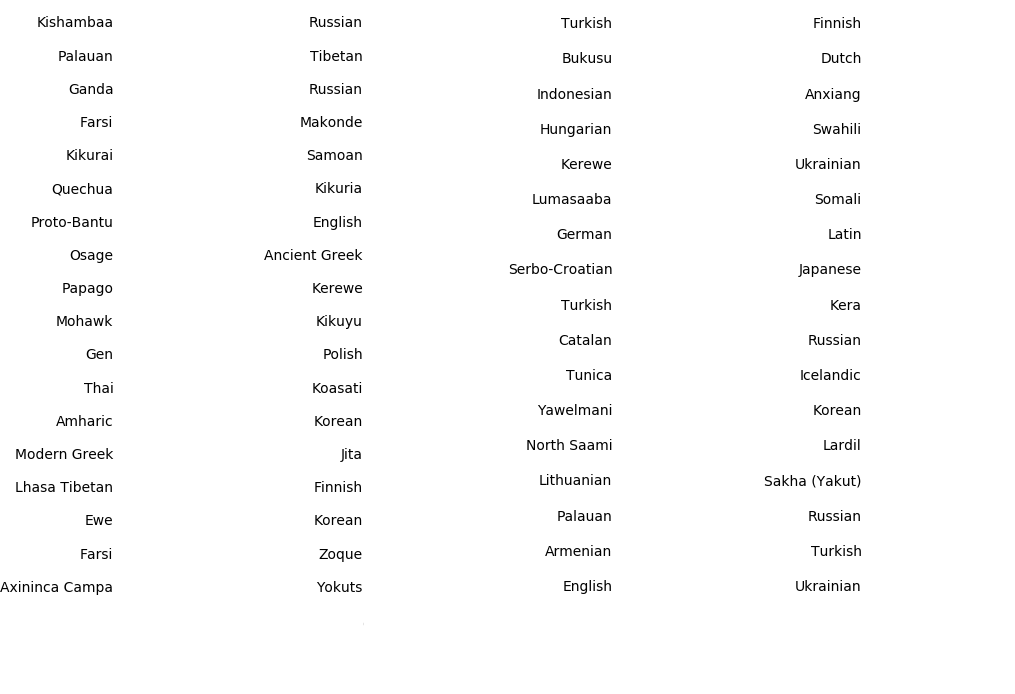
\includegraphics[width = \textwidth]{figures/percentage_solved_just_names}}
    \only<2>{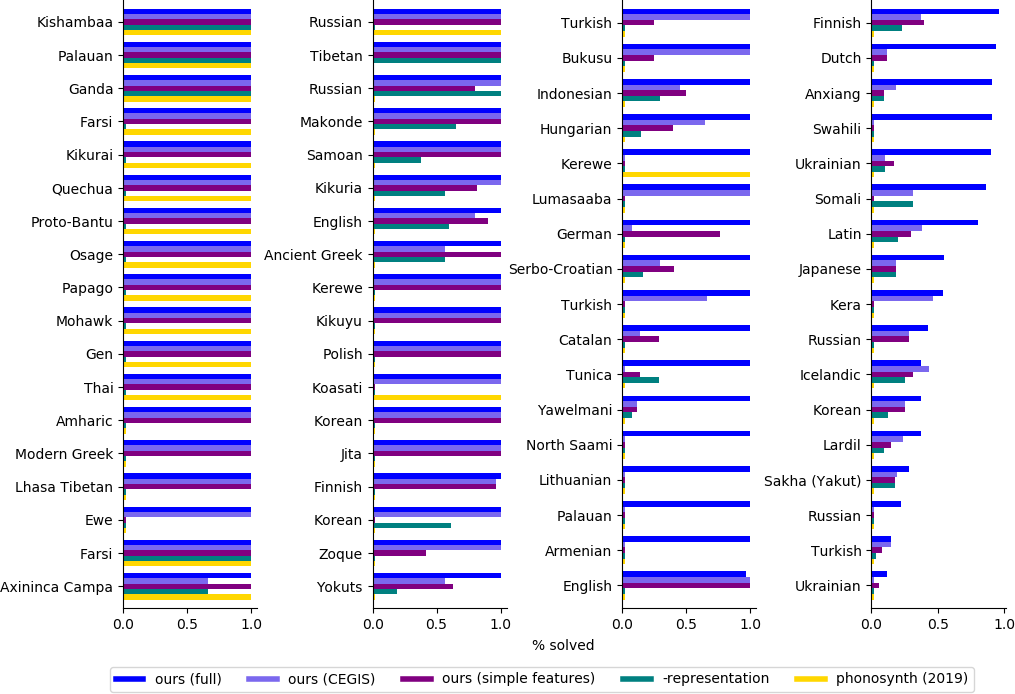
\includegraphics[width = \textwidth]{figures/percentage_solved}}
  }
%  \myPaper{\small Ellis, Albright, Solar-Lezama, Tenenbaum, O'Donnell. 2020.}
\end{frame}
\begin{frame}[fragile]{Distilling higher-level knowledge}
  \Wider[5em]{
    \begin{center}
      \begin{tikzpicture}[scale=2]
        \input{languageHierarchy.tex}
      \end{tikzpicture}
  \end{center}}
  \myPaper{\small Ellis, Albright, Solar-Lezama, Tenenbaum, O'Donnell. 2021.}
\end{frame}
\begin{frame}[fragile]{Distilling higher-level knowledge}
  \Wider[5em]{
    \begin{center}
      \begin{tikzpicture}[scale=2]
        \node[align=left] at (-2.2,0) {\textbf{dark}: we know it\\\textbf{light}: we wanna know it\\$\mathbf{A\to B}$: A makes B};
        \input{languageHierarchy2.tex}
      \end{tikzpicture}
  \end{center}}
  \myPaper{\small Ellis, Albright, Solar-Lezama, Tenenbaum, O'Donnell. 2021.}
\end{frame}
\begin{frame}[fragile]{Distilling higher-level knowledge}
  \Wider[5em]{
    \begin{center}
      \begin{tikzpicture}[scale=2]
        \node[align=left] at (-2.2,0) {\textbf{dark}: we know it\\\textbf{light}: we wanna know it\\$\mathbf{A\to B}$: A makes B};
        \input{languageHierarchy3.tex}
      \end{tikzpicture}
  \end{center}}
  \myPaper{\small Ellis, Albright, Solar-Lezama, Tenenbaum, O'Donnell. 2021.}
\end{frame}
\begin{frame}[fragile]{Distilling higher-level knowledge}
  \Wider[5em]{
    \begin{center}
      \begin{tikzpicture}[scale=2]
        \node[align=left] at (-2.2,0) {\textbf{dark}: we know it\\\textbf{light}: we wanna know it\\$\mathbf{A\to B}$: A makes B};
        \input{languageHierarchy4.tex}
      \end{tikzpicture}
  \end{center}}
  \myPaper{\small Ellis, Albright, Solar-Lezama, Tenenbaum, O'Donnell. 2021.}
\end{frame}
%% \begin{frame}{Distilling higher-level knowledge}
%%   \Wider[5em]{
%%     \begin{tabular}{rl}
%%       \begin{tabular}{c}
%%         Discovered\\ universal grammar \\schema
%%       \end{tabular}&
%%       \begin{tabular}{l}
%%         \multicolumn{1}{c}{\textbf{consonant/vowel distinction}}\\
%%         sounds$\gets$ [-vowel]\\
%%         sounds$\gets$ [+vowel]\\
%%         \emph{a set of sounds is commonly}\\\emph{ all consonants,}\\\emph{ or all vowels}
%%       \end{tabular}\\
%%       \begin{tabular}{c}
%%         w/o learned\\
%%         universal grammar
%%       \end{tabular}&
%%       Tibetan:\phantom{test}    \phonl{[-nasal]}{$\varnothing $}{\#}\\\\
%%       \begin{tabular}{c}
%%         w/ learned\\
%%         universal grammar
%%       \end{tabular}&
%%       \phantom{Tibetan:test} \phonb{[-vowel]}{$\varnothing $}{\# }{[-vowel]}

%% %% %    Kerewe&    \phonb{[ ]}{[ +hiTone ]}{[ +hiTone ] [ ] }{ [ ]}
%% %%   \end{tabular}&
      
%%     \end{tabular}
%% %%     \begin{tabular}{cll}
%% %%     \toprule&
%% %%   \multicolumn{1}{c}{Without learned universal grammar}&
%% %%   \multicolumn{1}{c}{With learned universal grammar}\\\midrule \\
%% %%   \begin{tabular}{l}
%% %%     \multicolumn{1}{c}{\textbf{consonant/vowel distinction}}\\
%% %%     sounds$\gets$ [-vowel]\\
%% %%     sounds$\gets$ [+vowel]\\
%% %%     \emph{a set of sounds is commonly}\\\emph{ all consonants,}\\\emph{ or all vowels}
%% %%   \end{tabular}&
%% %%   \begin{tabular}{rl}
%% %%     Tibetan&    \phonl{[-nasal]}{$\varnothing $}{\#}
%% %% %    Kerewe&    \phonb{[ ]}{[ +hiTone ]}{[ +hiTone ] [ ] }{ [ ]}
%% %%   \end{tabular}&
%% %%   \begin{tabular}{l}
%% %%     
%% %%   \end{tabular}
%% %%   \\\\\midrule   
%% %%   \begin{tabular}{l}
%% %%     \multicolumn{1}{c}{\textbf{nasal place assimilation}}\\
%% %%     $[\text{+nasal}]\to \alpha\text{place}$ / %\phonb{[+nasal]}{$\alpha$place}{\texttt{trigger}}{\phonfeat[c]{C\\$\alpha$place}}
%% %%     \underline{\phantom{aa}}\phonfeat[c]{C\\$\alpha$place}\\
%% %%     \emph{nasals (``n'', ``m'', ...) move to the place in the}\\
%% %%       \emph{ mouth where the next consonant is}
%% %%   \end{tabular}
%% %%   &
  
%% %%   \begin{tabular}{rl}    
%% %%     Bukusu&    \phonr{\textipa{\~n}}{$\alpha$place}{[$\alpha$place]}\\\\
%% %%   \end{tabular}
%% %%   &
%% %%   \begin{tabular}{l}
%% %%     \phonr{[+nasal]}{$\alpha$place}{\phonfeat[c]{C\\$\alpha$place}}\\\\
%% %%   \end{tabular}
%% %% \end{tabular}
%%   }
%% %\includegraphics[width = \textwidth]{phonology/universal}
%% \end{frame}



\begin{frame}{Lessons}

  Higher-level knowledge matters (``universal grammar''). Get the basics of the representation correct

  \vspace{1cm}

  But \emph{some} of this higher-level knowledge can be learned. You don't need millions of examples to learn it. But it's not a one-shot learning problem either

\end{frame}


\begin{frame}{}
  \begin{center}
    \begin{tabular}{l}
      {\textcolor{gray}{Higher-level Knowledge: Case study in linguistics}}\\
      {\textcolor{black}{Higher-level Knowledge: General program discovery}}
      \end{tabular}
  \end{center}
\end{frame}



\begin{frame}{Learning to write code} %Growing domain-specific knowledge}
  
  %  \Large
  Goal: acquire domain-specific knowledge needed to induce a class of programs


  
  \vspace{0.75cm}

  \Wider[4em]{
    \begin{itemize}
    \item Library of concepts (declarative knowledge; domain specific language) \\ %; generative model over programs)
      \item      Inference strategy (procedural knowledge; synthesis algorithm)
      \end{itemize}
  }

  \only<1>{
    \vspace{1cm}
    \centering\begin{tabular}{cccc}
      \person{Cathy Wong}{collaborators/cw}&
      \person{Max Nye}{collaborators/MaxNye}&
      \person{Mathias\\{\footnotesize Sable-Meyer}}{collaborators/French2}&
      \person{Lucas Morales}{collaborators/Lucas}
    \end{tabular}
  }
  
  \vspace{0.75cm}
  
  %% \visible<2>{
  %% \begin{tikzpicture}
  %%   \node(problem) at (0,0) {\includegraphics[width = 2cm]{figures/cubic.png}};
  %%   \node(synthesizer)[draw,align=center] at ([xshift=3cm]problem.east) {Learned \\program inducer};
  %%   \draw[->] (problem.east) -- (synthesizer.west);
  %%   \node(program)[draw, align=center] at ([xshift=3cm]synthesizer.east) {program:\\$f(x) = 0.3x^3+$\\$1.1x^2-2x+0.6$};
  %%   \draw[->] (synthesizer.east) -- (program.west);
  %% \end{tikzpicture}
  
  %%   \vspace{0.2cm}Concepts: $x^3$, $\alpha x + \beta$, etc\\Inference strategy: neurosymbolic search for programs}
  %% \renewcommand\code\texttt
  %%   \only<3>{
  %% \begin{tikzpicture}
  %%   \node(problem) at (0,0) {\includegraphics[width = 2cm]{figures/radialCircle.png}};
  %%   \node(synthesizer)[draw,align=center] at ([xshift=3cm]problem.east) {Learned \\program inducer};
  %%   \draw[->] (problem.east) -- (synthesizer.west);
  %%   \node(program)[draw, align=center] at ([xshift=3cm]synthesizer.east) {program:\\\code{(radial-symmetry 5}\\\code{ (circle 3))}};
  %%   \draw[->] (synthesizer.east) -- (program.west);
  %% \end{tikzpicture}
  
  %% \vspace{0.2cm}Concepts: \code{circle}, \code{radial-symmetry}, etc\\Inference strategy: neurosymbolic search for programs
  %%   }
\end{frame}


\begin{frame}{Library learning}
  \Wider[5em]{
    \begin{center}
      \begin{tabular}{cc}
        \includegraphics[height=\textheight]{figures/figureOneFinal1_primitives}&
        \includegraphics[height=\textheight]{figures/figureOneFinal1_problem}
      \end{tabular}
    \end{center}
  }
  \myPaper{Ellis, Wong, Nye, ..., Solar-Lezama, Tenenbaum. PLDI 2021.}
\end{frame}

\begin{frame}[t]{Library learning}
\Wider[5em]{  \begin{center}
    \begin{tabular}{ccc}
      \includegraphics[height=0.6\textheight]{figures/figureOneFinal1_primitives}&
      \phantom{testingtesting}&
      \includegraphics[height=0.6\textheight]{figures/figureOneFinal1_problem}
    \end{tabular}
\end{center}}
\myPaper{Ellis, Wong, Nye, ..., Solar-Lezama, Tenenbaum. PLDI 2021.}
\end{frame}


\begin{frame}{Library learning}
%  \centering
  
  \only<1>{  \Wider[5em]{\includegraphics[width = \textwidth]{figures/figureOneFinal1}}}
  \only<2>{  \Wider[5em]{\includegraphics[width = \textwidth]{figures/figureOneFinal2_layer1}}}
  \only<3>{  \Wider[5em]{\includegraphics[width = \textwidth]{figures/figureOneFinal2_layer1_exploded}}}
  \only<4>{  \Wider[5em]{\includegraphics[width = \textwidth]{figures/figureOneFinal2_layer1}}}
  \only<5>{  \Wider[5em]{\includegraphics[width = \textwidth]{figures/figureOneFinal2_layer2}}}
  \only<6>{  \Wider[5em]{\includegraphics[width = \textwidth]{figures/figureOneFinal2_layer2_exploded}}}
  \only<7>{  \Wider[5em]{\includegraphics[width = \textwidth]{figures/figureOneFinal2_layer2}}}
  \only<8>{  \Wider[5em]{\includegraphics[width = \textwidth]{figures/figureOneFinal2}}}
  \only<9>{  \Wider[5em]{\includegraphics[width = \textwidth]{figures/figureOneFinal2_exploded}}}
  \only<10>{  \Wider[5em]{\includegraphics[width = \textwidth]{figures/figureOneFinal3}}}
  \only<11>{  \Wider[5em]{\includegraphics[width = \textwidth]{figures/figureOneFinal3_explained_exploded}}}
  \only<12->{  \Wider[5em]{\includegraphics[width = \textwidth]{figures/figureOneFinal3_explained}}}
%  \only<12>{  \Wider[5em]{\includegraphics[width = \textwidth]{figures/figureOneFinal4}}}
  %  \only<5>{  \Wider[5em]{\includegraphics[width = \textwidth]{figures/figureOneFinal5}}}

  \visible<12->{Solution rewritten in initial primitives:

    \tiny\texttt{(lambda (x) (map (lambda (y) (car (fold (fold x nil (lambda (z u) (if (gt? (+ y 1) (length (fold x nil (lambda (v w) (if (gt? z v) (cons v w) w))))) (cons z u) u))) nil (lambda (a b) (if (nil? (fold (fold x nil (lambda (c d) (if (gt? (+ y 1) (length (fold x nil (lambda (e f) (if (gt? c e) (cons e f) f))))) (cons c d) d))) nil (lambda (g h) (if (gt? g a) (cons g h) h)))) (cons a b) b))))) (range (length x))))}}

  \visible<13>{\normalsize induced sort program found in $\leq 10$min. Brute-force search without learned library would take $\approx 10^{73}$ years }

  \myPaper{Ellis, Wong, Nye, ..., Solar-Lezama, Tenenbaum. PLDI 2021.}
  
\end{frame}

\begin{frame}{DreamCoder}
  \begin{itemize}
  \item   \textbf{Wake:} Solve problems by writing programs
  \item \textbf{Sleep:} Improve library and neural recognition model:
    \begin{itemize}
    \item \textbf{Abstraction sleep:} Improve library
      \item \textbf{Dream sleep:} Improve neural recognition model
    \end{itemize}
%  \item   Combines ideas from Wake-Sleep \& Exploration-Compression % \& Program analysis
  \end{itemize}

\hspace*{-0.4cm}\small cf. Helmholtz machine, wake/sleep neural network training algorithms
\end{frame}
\begin{frame}[t]{Library learning as Bayesian inference}
  %  \includegraphics[width = 11cm]{ecFigures/animation/EC.eps}
\centering  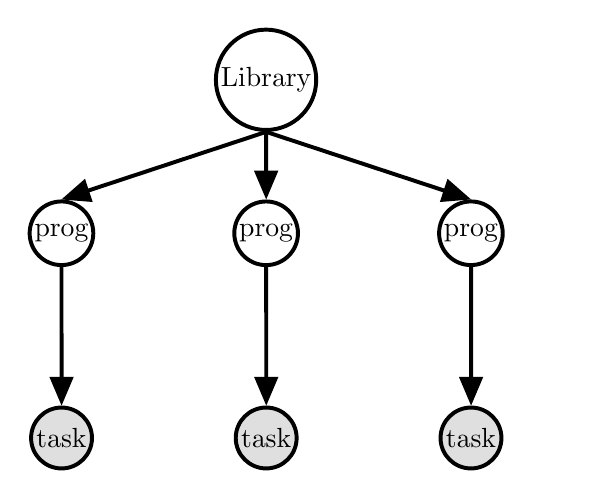
\begin{tikzpicture}[scale=1.3,line width=0.5mm]

  \node[latent,scale=1] at (3.5,3) (dx){Library};
  \node[latent,scale=1] at ([yshift=-1.5cm]dx) (zp){prog};
  \node[obs,scale=1] at ([yshift=-2cm]zp) (xp) {task};
  \node[latent,scale=1] at ([xshift=2cm]zp) (zp1){prog};
  \node[obs,scale=1] at ([xshift=2cm]xp) (xp1) {task};
  \draw [->] (zp1.south) -- (xp1.north);
  \draw [->] (dx.south) -- (zp1.north);
  %\draw [->,red] (xp1.east) to[out = 30,in = -30] node(nn){} (zp1.east);
%  \node at (nn) {\NeuralNetwork{0.5}};
  % HACK : "invisible" arrow to phantom and push to the left and align with next
  % slide
  \draw [->,red,opacity=0.0001] (xp1.east) to[out = 30,in = -30] node(nn){} (zp1.east);
  
  \node[latent,scale=1] at ([xshift=-2cm]zp) (zp1){prog};
  \node[obs,scale=1] at ([xshift=-2cm]xp) (xp1) {task};
  \draw [->] (zp1.south) -- (xp1.north);
  \draw [->] (dx.south) -- (zp1.north);
%  \draw [->,red] (xp1.east) to[out = 30,in = -30] node(nn){} (zp1.east);
%  \node at (nn) {\NeuralNetwork{0.5}};


%  \draw [->,red] (xp.east) to[out = 30,in = -30] node(nn){} (zp.east);
 % \node at (nn) {\NeuralNetwork{0.5}};
  \draw [->] (dx.south) -- (zp.north);
  \draw [->] (zp.south) -- (xp.north);


  %\node[shift={+(0,-1.7)}] at (nn) { $Q$  };

  \end{tikzpicture}
  

\vspace{0.5cm}
  
[Dechter et al, 2013]  [Liang et al, 2010] [Lake et al, 2015]

%\textbf{Dechter et al.}: Exploration-Compression. Inspiration for DreamCoder.

  %% \vfill
  %% Gray: Observed.\\
  %% White: Latent.\\
  %% Boxed (plate): Repeated.\\
  
\end{frame}
\newcommand{\NeuralNetwork}[1]{    \begin{tikzpicture}[x=2.5cm,y=1.25cm,transform canvas={scale=#1,shift={+(-1,2.5)}}]
      \tikzstyle{neuron}=[circle,fill=blue!50,minimum size=20pt]
      \fill[fill=white] (-0.25,-0.5) rectangle (2.25,-4.5);
      \node[rectangle] at (1,1) {};
      \foreach \name / \y in {1,...,4}
          \node[neuron] (I-\name) at (0,-\y) {};
      \foreach \name / \y in {1,...,3}
          \node[neuron] (H-\name) at (1,-\y-0.5) {};
      \foreach \name / \y in {1,...,4}
          \node[neuron] (O-\name) at (2,-\y) {};
      \foreach \source in {1,...,4}
          \foreach \dest in {1,...,3}
              \draw [-latex] (I-\source) -- (H-\dest);
      \foreach \source in {1,...,3}
          \foreach \dest in {1,...,4}
              \draw [-latex] (H-\source) -- (O-\dest);
    \end{tikzpicture}}
\begin{frame}[t]{Library learning as \alert{neurally-guided} Bayesian inference}
\centering  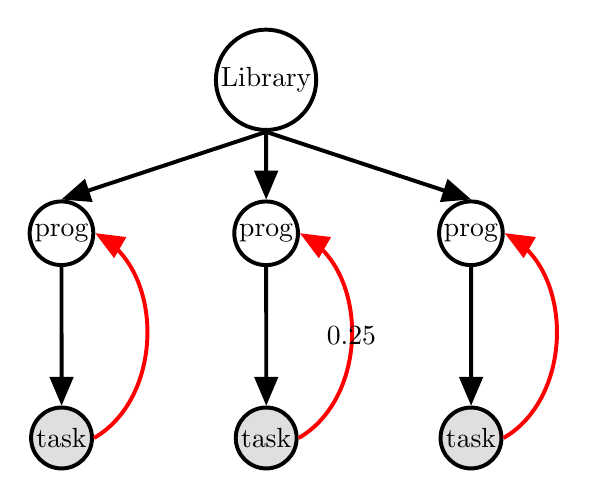
\begin{tikzpicture}[scale=1.3,line width=0.5mm]

  \node[latent,scale=1] at (3.5,3) (dx){Library};
  \node[latent,scale=1] at ([yshift=-1.5cm]dx) (zp){prog};
  \node[obs,scale=1] at ([yshift=-2cm]zp) (xp) {task};
  \node[latent,scale=1] at ([xshift=2cm]zp) (zp1){prog};
  \node[obs,scale=1] at ([xshift=2cm]xp) (xp1) {task};
  \draw [->] (zp1.south) -- (xp1.north);
  \draw [->] (dx.south) -- (zp1.north);
  \draw [->,red] (xp1.east) to[out = 30,in = -30] node(nn){} (zp1.east);
%  \node at (nn) {\NeuralNetwork{0.5}};
  
  \node[latent,scale=1] at ([xshift=-2cm]zp) (zp1){prog};
  \node[obs,scale=1] at ([xshift=-2cm]xp) (xp1) {task};
  \draw [->] (zp1.south) -- (xp1.north);
  \draw [->] (dx.south) -- (zp1.north);
  \draw [->,red] (xp1.east) to[out = 30,in = -30] node(nn){} (zp1.east);
%  \node at (nn) {\NeuralNetwork{0.5}};


  \draw [->,red] (xp.east) to[out = 30,in = -30] node(nn){} (zp.east);
  \node at (nn) {\NeuralNetwork{0.25}};
  \draw [->] (dx.south) -- (zp.north);
  \draw [->] (zp.south) -- (xp.north);


  %\node[shift={+(0,-1.7)}] at (nn) { $Q$  };

\end{tikzpicture}


\Wider[4em]{
  \begin{center}
    library learning via program analysis + \\
    new neural inference network for program synthesis + \\
    better program representation (Lisp+polymorphic types [Milner 1978])
  \end{center}
}
\myPaper{Ellis, Wong, Nye, ..., Solar-Lezama, Tenenbaum. PLDI 2021.}
\end{frame}
\newcommand{\NeuralNetwork}[1]{    \begin{tikzpicture}[x=2.5cm,y=1.25cm,transform canvas={scale=#1,shift={+(-1,2.5)}}]
      \tikzstyle{neuron}=[circle,fill=blue!50,minimum size=20pt]
      \fill[fill=teal!5!white] (-0.25,-0.5) rectangle (2.25,-4.5);
      \node[rectangle] at (1,1) {};
      \foreach \name / \y in {1,...,4}
          \node[neuron] (I-\name) at (0,-\y) {};
      \foreach \name / \y in {1,...,3}
          \node[neuron] (H-\name) at (1,-\y-0.5) {};
      \foreach \name / \y in {1,...,4}
          \node[neuron] (O-\name) at (2,-\y) {};
      \foreach \source in {1,...,4}
          \foreach \dest in {1,...,3}
              \draw [-latex] (I-\source) -- (H-\dest);
      \foreach \source in {1,...,3}
          \foreach \dest in {1,...,4}
              \draw [-latex] (H-\source) -- (O-\dest);
    \end{tikzpicture}}
\newcommand{\spiral}[2]{
  \draw[ultra thick,->] ([shift={#1}]-30:#2) arc [radius = #2, start angle = -30, end angle = 90];
  \draw[ultra thick,->] ([shift={#1}]-30:#2) arc [radius = #2, start angle = -30, end angle = 95];

  
      \draw[ultra thick,->] ([shift={#1}]90:#2) arc [radius = #2, start angle = 90, end angle = 210];
      \draw[ultra thick,->] ([shift={#1}]90:#2) arc [radius = #2, start angle = 90, end angle = 205];
      
      \draw[ultra thick,->] ([shift={#1}]210:#2) arc [radius = #2, start angle = 210, end angle = 340];
      \draw[ultra thick,->] ([shift={#1}]210:#2) arc [radius = #2, start angle = 210, end angle = 335];
}
\newcommand{\legend}{
  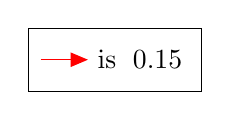
\begin{tikzpicture}
    \node at (0,0) (uses){is};
    \draw[->,red] ([xshift=-0.6cm]uses.west)  -- (uses.west);
    \node at ([xshift=0.4cm]uses.east) {\NeuralNetwork{0.15}};
    \draw[thin] (-1,-0.4) rectangle (1.2,0.4);
  \end{tikzpicture}
}

\begin{frame}{}
%  \myPaper{\footnotesize Ellis, Wong, Nye, ..., Solar-Lezama, Tenenbaum. PLDI 2021.}
  \centering
  \only<1>{

    \vspace{3cm}
    \includegraphics[width = 0.3\textwidth]{cycleGraphicalModel1.pdf}
  }

  

  \only<2>{\includegraphics[width = \textwidth]{cycleGraphicalModel2}}
  \only<3>{\includegraphics[width = \textwidth]{cycleGraphicalModel3}}
  \only<4>{\includegraphics[width = \textwidth]{cycleGraphicalModel4vl5}}
  \only<5>{\includegraphics[width = \textwidth]{cycleGraphicalModel4vl4}}
  \only<6>{\includegraphics[width = \textwidth]{cycleGraphicalModel4}}
  
  \only<7>{\includegraphics[width = \textwidth]{cycleGraphicalModelvl3}}
  \only<8>{\includegraphics[width = \textwidth]{cycleGraphicalModelvl2}}
  \only<9>{\includegraphics[width = \textwidth]{cycleGraphicalModelvl1}}
  \only<10>{\includegraphics[width = \textwidth]{cycleGraphicalModelvl}}
  %\only<6>{\includegraphics[width = \textwidth]{cycleGraphicalModelAbstraction}}
\end{frame}

%% \begin{frame}{DreamCoder's sleep cycles}
%% \tiny\begin{tikzpicture}[scale=0.55,line width=0.25mm]
%%     \draw[fill=teal!5!white] (-1.25,1.25) -- (13.25,1.25) -- (13.25,-4) -- (-1.25,-4) -- (-1.25,1.25);
%%     \node at (5.5,1.5) {\textsc{\textbf{Wake}}};

    
%%     \begin{scope}[shift={(0.5,0.5)}]
%%       \node[align=center] at (0,-0.5) (d){
%%         \begin{tabular}{l}
%%           \multicolumn{1}{c}{\textbf{Library}}\\
%%         \texttt{$f_1($x$)=$(+ x 1)}\\
%%         \texttt{$f_2($z$)=$(fold cons}\\
%%         \phantom{\texttt{$f_2($z$)$}}\texttt{(cons z nil))}\\
%%  $\cdots\cdots\cdots$
%%                 \end{tabular}};
%%       \node[align=center] at ([yshift = -2cm]d) (t){\textbf{Task}\\
%%                     \texttt{[7\, 2\, 3]}$\to$\texttt{[4 3 8]}         \\
%%             \texttt{[3\, 8]}$\to$\texttt{[9 4]}\\
%%             \texttt{[4\, 3\, 2]}$\to$\texttt{[3 4 5]} };

%%       \node at ([xshift = 1.25cm]t.east) (nn){\NeuralNetwork{0.1}};
%%       \node[align = center, text width = 1cm] at ([yshift = 0.7cm,xshift=0cm]nn.north) {\baselineskip=0pt  Recog. model\par};
%%       \draw [red,-{>[scale=0.2]}] (t.east) -- ([xshift = -0.5cm]nn.west);

%%       \node[draw,rounded corners, align=center, inner sep = 5] at ([xshift = 4.2cm,yshift = 1cm]t.east) (s){Neurally-Guided\\ Enumerative Search};

%%       \draw [red,->] ([xshift = 0.5cm]nn.east) -- ([yshift = -0.25cm]s.west);
%%       \draw [->,rounded corners,] (d.east) -- ([yshift = 2cm]nn.center) -- ([yshift = 0.25cm]s.west);

%%       \node[align=left] at ([xshift=3cm]s.east) (f) {\textbf{Programs for task:}\\
%%             \texttt{(map $f_1$ (fold $f_2$ nil x))}\\
%%          $\cdots\cdots\cdots$};
%%       \draw [->  ] (s.east) -- (f.west);

%%       \draw [->  ,rounded corners] (t.south) -- ([yshift = -0.5cm]t.south) -- ([yshift = -0.5cm] s.south |- t.south) -- (s.south);
%%     \end{scope}
    
%%     \begin{scope}[shift={(9.4,-3.5)},scale=0.6,line width=0.05mm]
%%       \node[obs,scale=0.7] at (3.5,3) (dx){Library};
%%       \node[latent,scale=0.7] at ([yshift=-1.7cm,xshift=0cm]dx) (zp){prog};
%%       \node[obs,scale=0.7] at ([yshift=-1.45cm]zp) (xp) {task};
%%       \node[latent,scale=0.7] at ([xshift=1.5cm]zp) (zp1){prog};
%%       \node[obs,scale=0.7] at ([xshift=1.5cm]xp) (xp1) {task};
%%       \draw [->] (zp1.south) -- (xp1.north);
%%       \draw [->] (dx.south) -- (zp1.north);
%%       \draw [->,red] (xp1.east) to[out = 30,in = -30] node(nn){} (zp1.east);
%%       \node[latent,scale=0.7] at ([xshift=-1.5cm]zp) (zp1){prog};
%%       \node[obs,scale=0.7] at ([xshift=-1.5cm]xp) (xp1) {task};
%%       \draw [->] (zp1.south) -- (xp1.north);
%%       \draw [->] (dx.south) -- (zp1.north);
%%       \draw [->] (dx.south) -- (zp.north);
%%       \draw [->] (zp.south) -- (xp.north);
%%       \draw [->,red] (xp1.east) to[out = 30,in = -30] node(nn){} (zp1.east);
%%       \draw [->,red] (xp.east) to[out = 30,in = -30] node(nn){} (zp.east);
%%     \end{scope}


%%     \node at (0,-4.75) {\textbf{\textsc{Sleep: Abstraction}}};
%%     \draw[fill=teal!5!white] (-3,-5) -- (3,-5) -- (3,-10) -- (5.5,-10) -- (5.5,-13) -- (-3,-13) -- (-3,-5);
%%     \node at (12,-4.75) {\textbf{\textsc{Sleep: Dreaming}}};
%%     \draw[fill=teal!5!white] (15,-5) -- (9,-5) -- (9,-10) -- (6.5,-10) -- (6.5,-13) -- (15,-13) -- (15,-5);

%%     \begin{scope}[shift={(9.5,-4.5)}]
%%       \node(dreaming) at (1,-1) {\underline{Fantasies}};
%%       \node[anchor=center] at ([yshift=-0.5cm]dreaming.south) (d){\textbf{Library}};
%%       \node at ([yshift=-1.75cm]d.south) (p1){program};
%%       \draw[squiggle,-> ] (d.south) -- node[sloped,above]{{ sample}} (p1.north);

%%       \node(replay) at ([xshift=2cm]dreaming.east) {\underline{Replays}};
%%       \node[anchor=center,align=center] at ([yshift=-0.5cm]replay.south) (d){\textbf{progs. for task}};
%%       \node at ([yshift=-1.75cm]d.south) (p1){program};
%%       \draw[squiggle,-> ] (d.south) -- node[sloped,above]{ sample} (p1.north);

%%       \node(p1) at (1.5,-6) {program};      
%%       \node at ([xshift = 2.0cm]p1.east) (t1){ task};
%%       \draw [-> ] (p1.east) -- node[above]{ run} (t1.west);
%%       \node(n) at ([yshift=-1.2cm,xshift=1.25cm]p1.south) {
%%         \NeuralNetwork{0.17}};
%%       \draw [->,red] (t1.south) to[out = -90,in = 0]  ([xshift=0.4cm]n.east);
%%       \draw [dashed] (p1.south) to[out=-120,in=180] node[above,fill=teal!5!white]{\color{black}Loss} ([xshift=-0.4cm]n.west);


%%       \node at ($(-0.25,0.5) + (p1.north)!0.5!(t1.north)$) {\underline{Train recognition model}};

%%       %% \node at ([xshift = 1.5cm]p1.east) (t1){ task};
%%       %% \draw [-> ] (p1.east) -- node[above]{ run} (t1.west);
%%       %% \node(n) at ([yshift=-1.2cm,xshift=0.4cm]p1.south) {
%%       %%   \NeuralNetwork{0.17}};
%%       %% \draw [->,red] (t1.south) to[out = -90,in = 0]  ([xshift=0.4cm]n.east);
%%       %% \draw [dashed] (p1.south) to[out=-120,in=180] node[above,fill=white]{\color{black}Loss} ([xshift=-0.4cm]n.west);

%%       \begin{scope}[shift={(-3.8,-8)},scale=0.6,line width=0.05mm]
%%         \node[obs,scale=0.4] at (3.5,3) (dx){L};
%%         \node[obs,scale=0.4] at ([yshift=-1.7cm,xshift=0cm]dx) (zp){p};
%%         \node[obs,scale=0.4] at ([yshift=-1.45cm]zp) (xp) {t};
%%         \node[obs,scale=0.4] at ([xshift=1.5cm]zp) (zp1){p};
%%         \node[obs,scale=0.4] at ([xshift=1.5cm]xp) (xp1) {t};
%%         \draw [->] (zp1.south) -- (xp1.north);
%%         \draw [->] (dx.south) -- (zp1.north);
%%         \draw [->,red] (xp1.east) to[out = 30,in = -30] node(nn){} (zp1.east);
%%         \node[obs,scale=0.4] at ([xshift=-1.5cm]zp) (zp1){p};
%%         \node[obs,scale=0.4] at ([xshift=-1.5cm]xp) (xp1) {t};
%%         \draw [->] (zp1.south) -- (xp1.north);
%%         \draw [->] (dx.south) -- (zp1.north);
%%         \draw [->] (dx.south) -- (zp.north);
%%         \draw [->] (zp.south) -- (xp.north);
%%         \draw [->,red] (xp1.east) to[out = 30,in = -30] node(nn){} (zp1.east);
%%         \draw [->,red] (xp.east) to[out = 30,in = -30] node(nn){} (zp.east);
%%       \end{scope}


%%       \end{scope}

%%     % memory consolidation
%%     \begin{scope}[shift={(-2,-4.5)}]

%%       %% defined routines for creating fragmented syntax trees
%%       \newcommand{\syntaxOne}[1]{
%%         \begin{tikzpicture}[scale=#1,line width=0.35mm]          
%%           \node(l1) at (0,0) {};
%%           \node[color=pop3](p1) at (-1,-1) {\texttt{+}};
%%           \node[color=pop3](n1) at (0.7,-0.9) {\texttt{1}};
%%           \node(x1) at (0,-1) {\texttt{1}};
%%           \draw[color=pop3] (l1.south) -- (p1.north);
%%           \draw[color=pop3] (l1.south) -- (n1.north);
%%           \draw[color=pop3] (-0.5,-0.45) -- (x1.north);

%%           \node(t) at (-0.5,0.5) {};
%%           \draw (l1.south) -- (t.south);
%%           \node(c) at (-1.5,-0.2) {\texttt{cons}};
%%           \draw (t.south) -- (c.north);
%%         \end{tikzpicture}
%%       }
%%       \newcommand{\syntaxTo}[1]{
%%         \begin{tikzpicture}[scale=#1,line width=0.35mm]          
%%             \node(l1) at (0,0) {};
%%             \node[color=pop3](p1) at (-1,-1) {\texttt{+}};
%%             \node[color=pop3](n1) at (0.7,-0.9) {\texttt{1}};
%%             \draw[color=pop3] (l1.south) -- (p1.north);
%%             \draw[color=pop3] (l1.south) -- (n1.north);
%%             \draw[color=pop3] (-0.5,-0.45) -- (0,-1);
%%             \node(c) at (-0.5,-1.5) {\texttt{car}};
%%             \node(z) at (0.5,-1.5) {\texttt{z}};
%%             \draw (0,-1) -- (c.north);
%%             \draw (0,-1) -- (z.north);
%%         \end{tikzpicture}
%%       }

%%       \node[align=center,anchor=center] at (0.4,-1.2) (f1){\textbf{ progs. for task 1}:\\\texttt{(+ (car z) 1)}};
%%       \node[align=center] at ([xshift = 1.75cm]f1.east) (f2){\textbf{  progs. for task 2}:\\\texttt{(cons (+ 1 1))}};
%%       \node(s1) at ([yshift=-0.5cm]f1.south) {\syntaxOne{0.5}};
%%       \node(s2) at ([yshift=-0.5cm]f2.south) {\syntaxTo{0.5}};
%%       \node(c)[align=center,rectangle, rounded corners, draw, minimum width = 1cm, minimum height = 0.5cm, anchor = north] at ($(s1.south)!0.5!(s2.south) + (0,-1)$) {Refactoring Algorithm};
%%       \draw [-> ] (s1.south) -- (s1.south|-c.north);
%%       \draw [-> ] (s2.south) -- (s2.south|-c.north);

      
%%       \node(d) at ([yshift = -1.8cm]c.south) {
%%         \begin{tikzpicture}[scale=0.5,line width=0.5mm]
%%           \node[align=center] at (0,0) {\textbf{new Library} w/ \texttt{(+ x 1)}:};
%%           \begin{scope}[shift={(0.6,-0.5)}]
%%             \node[pop3](p1) at (-1,-1) {\texttt{+}};
%%             \node[pop3](n1) at (0.6,-0.9) {\texttt{1}};
%%             \node[pop3](a) at (0,-1) {\texttt{ }};
%%             \draw[pop3] (0,0) -- (p1.north);
%%             \draw[pop3] (0,0) -- (n1.north);
%%             \draw[pop3] (-0.3,-0.3) -- (a.north);
%%           \end{scope}
%%       \end{tikzpicture}};
%%       \draw [-> ] (c.south) -- (d.north);



%%       \begin{scope}[shift={(4,-8)},scale=0.6,line width=0.05mm]
%%         \node[latent,scale=0.7] at (3.5,3) (dx){Library};
%%         \node[obs,scale=0.7] at ([yshift=-1.7cm,xshift=0cm]dx) (zp){prog};
%%         \node[obs,scale=0.7] at ([yshift=-1.45cm]zp) (xp) {task};
%%         \node[obs,scale=0.7] at ([xshift=1.5cm]zp) (zp1){prog};
%%         \node[obs,scale=0.7] at ([xshift=1.5cm]xp) (xp1) {task};
%%         \draw [->] (zp1.south) -- (xp1.north);
%%         \draw [->] (dx.south) -- (zp1.north);
%%         \node[obs,scale=0.7] at ([xshift=-1.5cm]zp) (zp1){prog};
%%         \node[obs,scale=0.7] at ([xshift=-1.5cm]xp) (xp1) {task};
%%         \draw [->] (zp1.south) -- (xp1.north);
%%         \draw [->] (dx.south) -- (zp1.north);
%%         \draw [->] (dx.south) -- (zp.north);
%%         \draw [->] (zp.south) -- (xp.north);
%%       \end{scope}


%%       \end{scope}


    
%%     %% center spiral
%%     \begin{scope}[shift={(3.25,-7.9)},scale=0.8]    
%%       \spiral{(3.5,1)}{3.5}
%%       \node[latent,scale=1] at (3.5,3) (dx){Library};
%%       \node[latent,scale=1] at ([yshift=-2cm,xshift=0cm]dx) (zp){prog};
%%       \node[obs,scale=1] at ([yshift=-1.45cm]zp) (xp) {task};
%%       \node[latent,scale=1] at ([xshift=2cm]zp) (zp1){prog};
%%       \node[obs,scale=1] at ([xshift=2cm]xp) (xp1) {task};
%%       \draw [->] (zp1.south) -- (xp1.north);
%%       \draw [->] (dx.south) -- (zp1.north);
%%       \draw [->,red] (xp1.east) to[out = 30,in = -30] node(nn){} (zp1.east);
      
%%       \node[latent,scale=1] at ([xshift=-2cm]zp) (zp1){prog};
%%       \node[obs,scale=1] at ([xshift=-2cm]xp) (xp1) {task};
%%       \draw [->] (zp1.south) -- (xp1.north);
%%       \draw [->] (dx.south) -- (zp1.north);
%%       \draw [->,red] (xp1.east) to[out = 30,in = -30] node(nn){} (zp1.east);


%%       \draw [->,red] (xp.east) to[out = 30,in = -30] node(nn){} (zp.east);
%%       \draw [->] (dx.south) -- (zp.north);
%%       \draw [->] (zp.south) -- (xp.north);

%%       \node at ([yshift=-0.6cm]xp.south) {\legend};

%%     \end{scope}    
%%   \end{tikzpicture}  

%% \end{frame}

%% \begin{frame}{}
%%   \only<1>{\includegraphics[width = \textwidth]{figures/compressionAnimation/1.jpg}}
%%   \only<2>{\includegraphics[width = \textwidth]{figures/compressionAnimation/2.jpg}}
%%   \only<3>{\includegraphics[width = \textwidth]{figures/compressionAnimation/3.jpg}}
%%   \only<4>{\includegraphics[width = \textwidth]{figures/compressionAnimation/4.jpg}}
%%   \only<5>{\includegraphics[width = \textwidth]{figures/compressionAnimation/5.jpg}}
%% %  \only<6>{\includegraphics[width = \textwidth]{figures/compressionAnimation/6.jpg}}
%%   \only<7>{\includegraphics[width = \textwidth]{figures/compressionAnimation/7.jpg}}
%%   \only<8>{\includegraphics[width = \textwidth]{figures/compressionAnimation/8.jpg}}
%%   \only<9>{\includegraphics[width = \textwidth]{figures/compressionAnimation/9.jpg}}
%%   \only<10>{\includegraphics[width = \textwidth]{figures/compressionAnimation/10.jpg}}
%%   \only<11>{\includegraphics[width = \textwidth]{figures/compressionAnimation/11.jpg}}
%%   \only<12>{\includegraphics[width = \textwidth]{figures/compressionAnimation/12.jpg}}
%%   \only<13>{\includegraphics[width = \textwidth]{figures/compressionAnimation/13.jpg}}
%%   \only<14>{\includegraphics[width = \textwidth]{figures/compressionAnimation/14.jpg}}
%%   \only<15>{\includegraphics[width = \textwidth]{figures/compressionAnimation/15.jpg}}
%%   \only<16>{\includegraphics[width = \textwidth]{figures/compressionAnimation/16.jpg}}
%%   \only<17>{\includegraphics[width = \textwidth]{figures/compressionAnimation/17.jpg}}
%%   \only<18>{\includegraphics[width = \textwidth]{figures/compressionAnimation/18.jpg}}
%%   \only<19>{\includegraphics[width = \textwidth]{figures/compressionAnimation/19.jpg}}
%%   \only<20>{\includegraphics[width = \textwidth]{figures/compressionAnimation/20.jpg}}
%%   \only<21>{\includegraphics[width = \textwidth]{figures/compressionAnimation/21.jpg}}
%%   \only<22>{\includegraphics[width = \textwidth]{figures/compressionAnimation/22.jpg}}
%%   \only<23>{\includegraphics[width = \textwidth]{figures/compressionAnimation/23.jpg}}
%%   \only<24>{\includegraphics[width = \textwidth]{figures/compressionAnimation/24.jpg}}
%%   \only<25>{\includegraphics[width = \textwidth]{figures/compressionAnimation/25.jpg}}
%%   \only<26>{\includegraphics[width = \textwidth]{figures/compressionAnimation/26.jpg}}
%% \end{frame}
\newcommand{\abstractionTree}[2]{
  \smallTree{#1}{#2}{+}{$x$}{$x$};
  \node(a#1) at ([yshift=0.5cm]root#1.south) {$\lambda x$};

  \draw (a#1.south) -- (root#1.south);  
  }
\newcommand{\smallTree}[5]{
  \node(root#1) at (#2) {};
  \node[anchor=north](r#1) at ([xshift=0.5cm,yshift=-0.5cm]root#1) {#5};
  \node(l#1) at ([xshift=-0.5cm,yshift=-0.5cm]root#1) {};
  \node(ll#1) at ([xshift=-0.5cm,yshift=-0.5cm]l#1) {#3};
  \node(lr#1) at ([xshift=0.5cm,yshift=-0.5cm]l#1) {#4};

  \draw (root#1.south) -- (r#1.north);
  \draw (root#1.south) -- (l#1.north);
  \draw (l#1.north) -- (ll#1.north);
  \draw (l#1.north) -- (lr#1.north);
}
\newcommand{\appliedTree}[6]{
  \smallTree{#1}{#2}{#3}{#4}{#5};
  \node(a#1) at ([yshift=0.5cm]root#1.south) {$\lambda x$};
  \node(ar#1) at ([xshift=0.5cm,yshift=0.4cm]a#1.north) {};
  \node[anchor=north](argument#1) at ([xshift=1cm]a#1.north) {#6};

  \draw (a#1.south) -- (root#1.south);
  \draw (argument#1.north) -- (ar#1.south);
  \draw (a#1.north) -- (ar#1.south);
}
\newcommand{\chooseAny}[4]{
  \node[anchor=north](any#1) at (#2) {\textsc{\small Any}};
  \node(anyl#1) at ([xshift=-0.25cm,yshift=-0.5cm]any#1.south) {#3};
  \node(anyr#1) at ([xshift=0.25cm,yshift=-0.5cm]any#1.south) {#4};
  \draw (any#1.south)--(anyl#1.north);
  \draw (any#1.south)--(anyr#1.north);  
}
\newcommand{\chooseTreeTiny}[3]{
  \node(a#1) at (#2) {$\lambda z$};
  \node(ar#1) at ([xshift=0.5cm,yshift=0.4cm]a#1.north) {};
  \node[anchor=north](argument#1) at ([xshift=1cm]a#1.north) {#3};

  \chooseAny{any#1}{[yshift=-0.2cm]a#1.south}{#3}{$z$}

  \draw (a#1.south) -- (anyany#1.north);
  \draw (argument#1.north) -- (ar#1.south);
  \draw (a#1.north) -- (ar#1.south);
}  

\newcommand{\chooseTreeSmall}[7]{
  \node(root#1) at (#2) {};
  \node[anchor=north](r#1) at ([xshift=0.5cm,yshift=-0.5cm]root#1) {#5};
  \node(l#1) at ([xshift=-0.5cm,yshift=-0.5cm]root#1) {};
  \chooseAny{any#1}{[xshift=-0.5cm,yshift=-0.5cm]l#1}{#3}{#4};
  \draw (l#1.north) -- (anyany#1.north);
%  \node(ll#1) at ([xshift=-0.5cm,yshift=-0.5cm]l#1) {};
  \node(lr#1) at ([xshift=0.5cm,yshift=-0.5cm]l#1) {#5};

  \draw (root#1.south) -- (r#1.north);
  \draw (root#1.south) -- (l#1.north);
  \draw (l#1.north) -- (lr#1.north);

  \node(a#1) at ([yshift=0.5cm]root#1.south) {$\lambda y$};
  \node(ar#1) at ([xshift=0.5cm,yshift=0.4cm]a#1.north) {};
  \node[anchor=north](argument#1) at ([xshift=1cm]a#1.north) {#7};

  \draw (a#1.south) -- (root#1.south);
  \draw (argument#1.north) -- (ar#1.south);
  \draw (a#1.north) -- (ar#1.south);
}
\newcommand{\chooseTree}[6]{
  \node(root#1) at (#2) {};
  \chooseAny{anyl#1}{[xshift=1cm,yshift=-0.8cm]root#1}{#4}{#5};
  \draw (root#1.south) -- (anyanyl#1.north);  
  \node(l#1) at ([xshift=-0.75cm,yshift=-0.75cm]root#1) {};
  \node(ll#1) at ([xshift=-0.75cm,yshift=-0.75cm]l#1) {#3};
  \chooseAny{anyr#1}{[xshift=0.5cm,yshift=-0.5cm]l#1}{#4}{#5};
  \draw (l#1.north) -- (anyanyr#1.north);

  \draw (root#1.south) -- (l#1.north);
  \draw (l#1.north) -- (ll#1.north);


  \node(a#1) at ([yshift=0.5cm]root#1.south) {$\lambda x$};
  \node(ar#1) at ([xshift=0.5cm,yshift=0.4cm]a#1.north) {};
  \node[anchor=north](argument#1) at ([xshift=1cm]a#1.north) {#6};

  \draw (a#1.south) -- (root#1.south);
  \draw (argument#1.north) -- (ar#1.south);
  \draw (a#1.north) -- (ar#1.south);
}
\newcommand{\chooseTreeCompact}[6]{
  \node(root#1) at (#2) {};
  \chooseAny{anyl#1}{[xshift=0.75cm,yshift=-0.5cm]root#1}{#4}{#5};
  \draw (root#1.south) -- (anyanyl#1.north);  
  \node(l#1) at ([xshift=-0.5cm,yshift=-0.5cm]root#1) {};
  \node(ll#1) at ([xshift=-0.5cm,yshift=-0.5cm]l#1) {#3};
  \chooseAny{anyr#1}{[xshift=0.3cm,yshift=-0.3cm]l#1}{#4}{#5};
  \draw (l#1.north) -- (anyanyr#1.north);

  \draw (root#1.south) -- (l#1.north);
  \draw (l#1.north) -- (ll#1.north);


  \node(a#1) at ([yshift=0.5cm]root#1.south) {$\lambda x$};
  \node(ar#1) at ([xshift=0.5cm,yshift=0.4cm]a#1.north) {};
  \node[anchor=north](argument#1) at ([xshift=1cm]a#1.north) {#6};

  \draw (a#1.south) -- (root#1.south);
  \draw (argument#1.north) -- (ar#1.south);
  \draw (a#1.north) -- (ar#1.south);
}
  
  





\begin{frame}{DreamCoder Domains}
  \Wider[5em]{
    \only<1>{\includegraphics[width = \textwidth]{figures/manyDomainsLarger.png}}%{statement/taskbar2_expended.png}}
    \only<2>{\includegraphics[width = \textwidth]{figures/manyDomainsSelectedNoTower.png}}%statement/taskbar2_selected.png}}
  }
  \myPaper{\small Ellis, Wong, Nye, ..., Solar-Lezama, Tenenbaum. PLDI 2021.}
\end{frame}

\begin{frame}{LOGO Turtle Graphics}
  30 out of 160 tasks
  \includegraphics[width = \textwidth]{dc/logoTasks30.png}
  \myPaper{\small Ellis, Wong, Nye, ..., Solar-Lezama, Tenenbaum. PLDI 2021.}
\end{frame}

\begin{frame}{LOGO Turtle Graphics -- learning an interpretable library}
  \Wider[5em]{
    \only<1>{\includegraphics[width = \textwidth]{dc/logo_kathy.png}}
    \only<2>{\includegraphics[width = \textwidth]{dc/logo_kathy_exploded1.png}}
    \only<3>{\includegraphics[width = \textwidth]{dc/logo_kathy_exploded2.png}}
    \only<4>{\includegraphics[width = \textwidth]{dc/logo_kathy_exploded3.png}}
    \only<5->{\includegraphics[width = \textwidth]{dc/logo_kathy.png}}
      
  }

  \only<6>{
  \messageOverlay{
    \begin{tabular}{rl}
    circle$(r)$
    &\raisebox{-.5\height}{\includegraphics[width = 0.3\textwidth]{dc/logo_primitives/circle_negative.png}}\\
    arc$(n,\ell,\theta)$
    &\raisebox{-.5\height}{\includegraphics[width = 0.3\textwidth]{../dreamcoder/figures/logo_primitives/arc/arc.png}}
    %% polygon$(n,\ell)$
    %% &\raisebox{-.5\height}{\includegraphics[width = 0.3\textwidth]{dc/logo_primitives/polygon_negative.png}}
  \end{tabular}
  }}
  \only<5>{
    \messageOverlay{\begin{tabular}{c}
    radial symmetry$(n,\text{body})$\\
    \includegraphics[width = 0.35\textwidth]{dc/rotationalmontage_negative.png}
  \end{tabular}}
  }
  \myPaper{\small Ellis, Wong, Nye, ..., Solar-Lezama, Tenenbaum. PLDI 2021.}
\end{frame}

\begin{frame}{What does DreamCoder dream of? (before learning)}
%  \emph{before} learning:
  \Wider[5em]{
    \begin{center}
      \includegraphics[height=\textheight]{dc/dreams/beforeLearning36}
    \end{center}
  }
%  \myPaper{Ellis, Wong, Nye, ..., Solar-Lezama, Tenenbaum. PLDI 2021.}  
  %  \includegraphics[height=3cm]{dc/dreams/cherry_picked/montageSeptember14}    
%    \end{tabular}}
    %% \only<2>{\begin{tabular}{lll}
    %%     before learning&&after learning\\
    %%     \includegraphics[width = 0.4\textwidth]{dc/dreams/appendixlogoinitial.png}&&
    %%     \includegraphics[width = 0.4\textwidth]{dc/dreams/appendixlogofinal.png}
    %%     \end{tabular}}
\end{frame}

\begin{frame}{What does DreamCoder dream of? (after learning)}
%  \emph{after} learning:
  \Wider[4em]{
    \begin{center}
      \includegraphics[height=\textheight]{figures/postDreams6}
    \end{center}
  }
%  \myPaper{Ellis, Wong, Nye, ..., Solar-Lezama, Tenenbaum. PLDI 2021.}  

%    \end{tabular}}
    %% \only<2>{\begin{tabular}{lll}
    %%     before learning&&after learning\\
    %%     \includegraphics[width = 0.4\textwidth]{dc/dreams/appendixlogoinitial.png}&&
    %%     \includegraphics[width = 0.4\textwidth]{dc/dreams/appendixlogofinal.png}
    %%     \end{tabular}}
\end{frame}

%% \begin{frame}{Planning to build towers}
%%   \myPaper{\small Ellis, Wong, Nye, ..., Solar-Lezama, Tenenbaum. PLDI 2021.}
%%   \Wider[5.5em]{
%%     \footnotesize
%%     \begin{tabular}{l}
%%       {example tasks (112 total)}\\
%%       \includegraphics[clip, trim = 0 0cm 0 2.9cm,width = 0.9\textwidth]{dc/tower_montage_21_negative.png}\\\\

%%     \end{tabular}
%%     \pause
%%     \begin{tabular}{l}
%%       {learned library routines ($\approx $ 20 total)}\\
%%       \begin{tabular}[t]{rlrl}
%%         arch$(h)$&%\begin{tabular}{l}
%%         \raisebox{-.1\height}{\includegraphics[width = 0.25\textwidth]{dc/tower/tower_dsl_towerArch.png}}&
%%         %\end{tabular}&
%%         pyramid$(h)$&
%%         \raisebox{-.1\height}{\includegraphics[width = 0.25\textwidth]{dc/tower/tower_dsl_pyramid.png}}
%%         \\
%%         wall$(w,h)$&
%%         \raisebox{-.3\height}{\includegraphics[width = 0.25\textwidth]{dc/tower/tower_dsl_bricks.png}}
%%         &%\\\\
%%         %% stairs$(h)$&\begin{tabular}{l}
%%         %%   \includegraphics[width = 0.25\textwidth]{dc/tower/tower_dsl_staircase.png}
%%         %% \end{tabular}\\\\
%%         \phantom{bbb}bridge$(w,h)$&
%%         \raisebox{-.3\height}{\includegraphics[width = 0.25\textwidth]{dc/tower/tower_dsl_bridge.png}}
%%         %\\\\\\
%%       \end{tabular}\\\\

%%   \end{tabular}}

%%   %% \pause

%%   %% \messageOverlay{
%%   %%   \begin{tabular}{ll}
%%   %%         \textbf{dreams before learning}&\textbf{dreams after learning}\\
%%   %%         \begin{tabular}{c}
%%   %%           \includegraphics[clip,trim = 0 4.5cm 0 0cm,width = 0.4\textwidth]{dc/tower/dreams/cherry_montage_initial_20.png}
%%   %%         \end{tabular}\phantom{testing}&
%%   %%         \begin{tabular}{c}
%%   %%           \includegraphics[clip,trim = 0 4.5cm 0 0cm,width = 0.4\textwidth]{dc/tower/dreams/cherry_montage_final.png}
%%   %%           \end{tabular}
%%   %%         \\\\
%%   %%     \end{tabular}
%%   %% }
%% \end{frame}

%% \begin{frame}{Dreams before learning}
%%   \includegraphics[clip,trim = 0 4.5cm 0 0cm,width = \textwidth]{dc/tower/dreams/cherry_montage_initial_20.png}
%% %  \myPaper{\small Ellis, Wong, Nye, ..., Solar-Lezama, Tenenbaum. PLDI 2021.}
%% \end{frame}

%% \begin{frame}{Dreams after learning}
%%   \includegraphics[clip,trim = 0 4.5cm 0 0cm,width = \textwidth]{dc/tower/dreams/cherry_montage_final.png}
%% %  \myPaper{\small Ellis, Wong, Nye, ..., Solar-Lezama, Tenenbaum. PLDI 2021.}
%% \end{frame}


\begin{frame}{Learning dynamics}
  \phantom{
  \small baselines: Exploration-Compression, EC [Dechter et al. 2013]
    \small \phantom{baselines: }neural program synthesis, RobustFill [Devlin et al. 2017]\phantom{otest}
    \small \phantom{baselines: }24 hours of brute-force enumeration
    }
  \begin{tabular}{lr}
    \begin{tabular}{l}
    \only<1>{\includegraphics[height = 2.29cm]{figures/revisedLearningCurves/tower_hits_ws_average_pretty_small_yl_stage1.png}}
    %    \only<2>{\includegraphics[height = 2.29cm]{figures/revisedLearningCurves/tower_hits_ws_average_pretty_small_yl_stage2.png}}
    \only<2>{\includegraphics[height = 2.29cm]{figures/tower_hits_ws_average_pretty_small_yl_ablationStage.png}}
%    \only<3>{\includegraphics[height = 2.29cm]{figures/revisedLearningCurves/tower_hits_ws_average_pretty_small_yl_stage3.png}}
  \end{tabular}

    &

    \begin{tabular}{l}
      \only<2>{\includegraphics[width = 3cm]{figures/revisedLearningCurves/curveLegendTruncated.png}}
  \end{tabular}
  \end{tabular}

  



  %% }
  %% }
  \myPaper{\small Ellis, Wong, Nye, ..., Solar-Lezama, Tenenbaum. PLDI 2021.}
\end{frame}

\begin{frame}{Synergy between Dreaming, Discovery, \& Higher-level knowledge}
  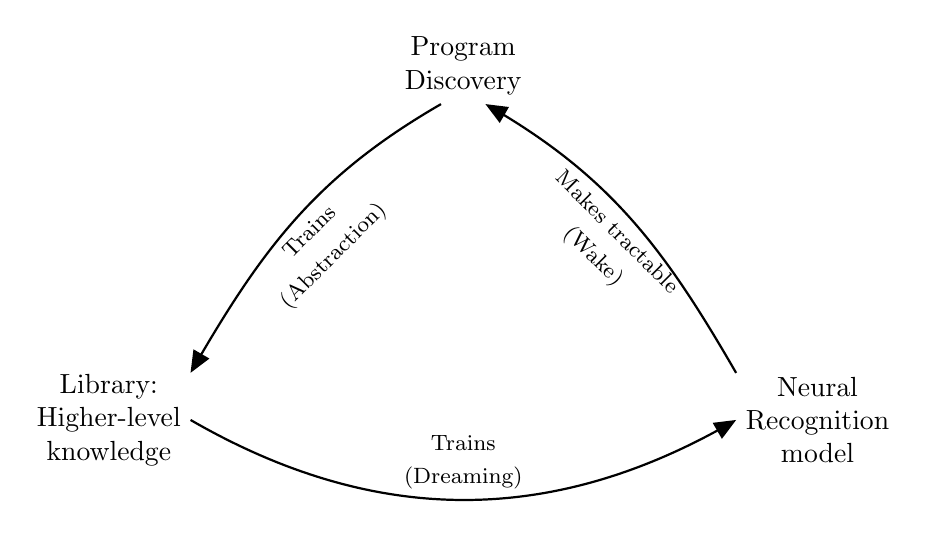
\begin{tikzpicture}[scale=1.5]
    {
    \begin{scope}[shift = {(1,-1)}]
    \node[align = center](synthesis) at (6,4) {Program\\Discovery};
    \node[align = center](Library) at (3,1) {Library:\\Higher-level\\knowledge};
    \node[align = center](recognitionModel) at (9,1) {Neural\\Recognition \\model};

    \visible<2->{
      \draw [->,thick] (synthesis.-120) to[out = -150,in = 60] node[below,rotate = 45,align = center]{{\footnotesize Trains}\\{\footnotesize (Abstraction)}} (Library.30);
    }
    \visible<3->{
%      \draw [->,thick] (synthesis.-60) to[out = -30,in = 120] node[below,rotate=-45,align = center]{{\footnotesize Trains}\\{\footnotesize (Dreaming)}} (recognitionModel.150);
      \draw [->,thick] (Library.east) to[out = -30,in = 210] node[above, align = center]{{\footnotesize Trains}\\{\footnotesize (Dreaming)}} (recognitionModel.west);    
    }


    \visible<4->{
      \draw [->,thick] (recognitionModel.150) to[in = -30,out = 120] node[below,rotate=-45,align = center]{{\footnotesize Makes tractable}\\{\footnotesize (Wake)}} (synthesis.-60);
    }

    %% \visible<5->{
    %%   \draw [->,thick,dashed] (recognitionModel.north) to[out = 90,in = 0] node[fill=backgroundBeige,inner sep=1pt,align = center]{{\footnotesize Trains}\\{\footnotesize (Dreaming)}} (synthesis.east);
    %%   \draw [->,thick,dashed] (Library.north) to[out = 90,in = 180] node[fill=backgroundBeige,inner sep=0pt,align = center]{\footnotesize{Inductive bias}\\\footnotesize{(Wake)}
    %%   } (synthesis.west);
    %% }

  \end{scope}}
    \end{tikzpicture}
  \myPaper{\small Ellis, Wong, Nye, ..., Solar-Lezama, Tenenbaum. PLDI 2021.}
\end{frame}

\begin{frame}{Evidence for dreaming bootstrapping better libraries}
  \begin{center}
    \begin{tabular}{c}
      %        \multicolumn{1}{l}{\textbf{B}}\\
      \only<1>{\includegraphics[height = 0.3\textwidth]{figures/depthVersusAccuracy_revision_MEAN_blue.png}}
    \only<2->{\includegraphics[height = 0.3\textwidth]{figures/depthVersusAccuracy_revision_MEAN.png}}
\\\\
 \visible<2->{\includegraphics[height = 1cm]{figures/revisedLearningCurves/scatterLegend.png}}
    \end{tabular}

    
    Darker: Early in learning

    Brighter: Later in learning

  \end{center}
  
  \myPaper{\small Ellis, Wong, Nye, ..., Solar-Lezama, Tenenbaum. PLDI 2021.}
\end{frame}



\begin{frame}{}

  {\huge
    From learning libraries,\phantom{tttesttesttest} \phantom{Fr} to learning languages}

  \vspace{2cm}

  \Wider[4em]{
    \visible<3>{\Large 1950's Lisp $\to $  }\visible<2->{\Large modern functional programming $\to $ physics}
  }
\end{frame}

\begin{frame}{}
  \begin{center}
    \includegraphics[width = 0.8\textwidth]{figures/PhysicsFormulas}
   \end{center}
\end{frame}

\begin{frame}{Growing languages for vector algebra and physics}
  \myPaper{\small Ellis, Wong, Nye, ..., Solar-Lezama, Tenenbaum. PLDI 2021.}
  \Wider[5em]{
    \only<1>{\includegraphics[width = \textwidth]{figures/physicsAnimation7}}
    \only<2>{\includegraphics[width = \textwidth]{figures/physicsAnimation6}}
    \only<3>{\includegraphics[width = \textwidth]{figures/physicsAnimation5}}
%    \only<4>{\includegraphics[width = \textwidth]{figures/physicsAnimation4}}
    \only<4>{\includegraphics[width = \textwidth]{figures/physicsAnimation3}}
    \only<5>{\includegraphics[width = \textwidth]{figures/physicsAnimation2}}
    \only<6>{\includegraphics[width = \textwidth]{figures/physicsAnimation1}}
  }
\end{frame}

\begin{frame}{Growing a language for recursive programming}
  \myPaper{\small Ellis, Wong, Nye, ..., Solar-Lezama, Tenenbaum. PLDI 2021.}\Wider[5em]{\only<1>{\includegraphics[width = \textwidth]{figures/mcCarthyAnimation5}}
    \only<2>{\includegraphics[width = \textwidth]{figures/mcCarthyAnimation4}}
    \only<3>{\includegraphics[width = \textwidth]{figures/mcCarthyAnimation3}}
    \only<4->{\includegraphics[width = \textwidth]{figures/mcCarthyAnimation2}}
%    \only<5>{\includegraphics[width = \textwidth]{figures/mcCarthyAnimation1}}
  }

  \vspace{-0.5cm}
  
  \visible<6>{\textbf{\Large 1 year of compute. 5 days on 64 CPUs.}}
  
  \visible<5->{
    \begin{tabular}{cc}
      \begin{tabular}{c}
        \includegraphics[width = 2cm]{figures/origamiCrane}
        \end{tabular}&\normalsize Origami Programming: Jeremy Gibbons, 2003
    \end{tabular}
  }
\end{frame}

\begin{frame}{Lessons}

  Programs as a knowledge representation for discovery problems

  \pause

  \vspace{1cm}


  Higher-level knowledge makes program synthesis tractable

  \pause

  \vspace{1cm}

  Higher-level knowledge makes these programs more interpretable
\end{frame}

\begin{frame}{}

  \Huge\centering

  \texttt{the end.}

\end{frame}


\begin{comment}
  \begin{frame}{What's far off, but worthwhile?}
    What kinds of future machines could learn all this?

    \vspace{1cm}

    \Wider[5em]{
      \begin{center}
        \only<1>{\begin{tabular}{ccc}
            using new devices&play&coding\\
            \includegraphics[height = 2cm]{figures/noodles}&
            \includegraphics[height = 2cm]{figures/childPlaying}&
            \includegraphics[height = 2cm]{../ecPaper/figures/1975.png}\\
            language&science&design\\%&engineering\\
            \includegraphics[height = 2cm]{figures/acquisition}&
            \includegraphics[height = 2cm]{figures/blackboard}&
            \includegraphics[height = 2cm]{figures/textile2}
            %      \includegraphics[height = 2cm]{figures/primitiveTools}\\
        \end{tabular}}
      \end{center}
    }
    

    

  \end{frame}
\end{comment}

\begin{frame}
\centering
  \begin{tabular}{cc}
    \bigPerson{Josh Tenenbaum}{collaborators/Josh}&
    \bigPerson{Armando Solar-Lezama}{collaborators/Armando}&
    \end{tabular}
\end{frame}

\renewcommand{\person}[2]{\closex{0.2}{\begin{tabular}{c}
    {\footnotesize #1}\\
    \includegraphics[width = 2.3cm]{#2}
\end{tabular}}}

\begin{frame}%{Collaborators}
\Wider[6em]{\centering \closey{0}{ \begin{tabular}{ccccc}
    \person{Evan Pu}{collaborators/haircut}&
    \person{Lucas Tian}{collaborators/LucasT}&
    \person{Marta Kryven}{collaborators/Marta}&
%    \person{Adam Albright}{collaborators/Adam}&
    \person{Chris Yang}{collaborators/Chris}&
    \person{Ronald Alvarez}{collaborators/Ronald}\\
%        \person{Josh Rule}{collaborators/jr}\\
    \person{Max Nye}{collaborators/MaxNye}& 
    \person{Cathy Wong}{collaborators/cw}&
%    \person{Jiajun Wu}{collaborators/jw}    &
%    \person{Dan Ritchie}{collaborators/Daniel}&
    \person{Kliment\\{\footnotesize Serafimov}}{collaborators/ks}&
    \person{Eyal Dechter}{collaborators/eyal}&
    \person{Mathias\\{\footnotesize Sable-Meyer}}{collaborators/French}\\
    \person{Lucas Morales}{collaborators/Lucas}&
    \person{Tao Du}{collaborators/tao}&
    \person{Felix Sosa}{collaborators/Felix}&
%    \person{Tim O'Donnell}{collaborators/Timothy}\\
%    \person{Owen Lewis}{collaborators/Owen}&
%    \person{Sumit Gulwani}{collaborators/sg}&
    \person{Sam Tenka}{collaborators/st}&
    \person{Julio\\{\footnotesize Cortazar}}{collaborators/Julio.jpg} 
    \end{tabular}}}  
\end{frame}

\begin{frame}{thank you...}
  family

  \begin{tabular}{cccc}
    \includegraphics[width = 2cm]{collaborators/family/1}
    &    \includegraphics[width = 2cm]{collaborators/family/2}
    &    \includegraphics[width = 2.5cm]{collaborators/family/3}
    &    \includegraphics[width = 2cm]{collaborators/family/g}
  \end{tabular}

  \vspace{1cm}

  MIT Brain and Cognitive Sciences

  \vspace{1cm}

  twitch viewers

\end{frame}

\begin{frame}{}

  \Huge\centering

  \texttt{the end.}

  \end{frame}

\begin{frame}
  \only<1>{\includegraphics[width = \textwidth]{cycleGraphicalModel5}}
  \only<2>{\includegraphics[width = \textwidth]{cycleGraphicalModelRecognition}}
\end{frame}

\begin{frame}[t]{Neural recognition model guides search}
  \vspace{1.2cm}
  \begin{tikzpicture}
    \node(t) at (0,0) {task};
    \node(n) at ([xshift=2cm]task.east) {
      \NeuralNetwork{0.17}};
    \node(p) at ([xshift=2cm]n.east) {program};
    \draw[thick,->] (t.east) -- ([xshift=-0.4cm]n.west);
    \draw[thick,->] ([xshift=0.4cm]n.east) -- (p.west);

    %% \node(n1) at ([yshift=-2cm]t.south) {\phantom{.}};
    %% \node[anchor=north west,align=left](c1) at ([xshift=0.5cm,yshift=0.3cm]n1.east) {\phantom{is a \textbf{``bigram'' model over syntax trees}}\\\phantom{test}\\\phantom{test}}\\\phantom{test}};
  \end{tikzpicture}

\end{frame}
\begin{frame}[t]{Neural recognition model guides search}
  \vspace{1cm}
  \begin{tikzpicture}
    \node(t) at (0,0) {task};
    \node(n) at ([xshift=2cm]task.east) {
      \NeuralNetwork{0.17}};
    \node(d) at ([xshift=2cm]n.east) {distribution};
    \draw[thick,->] (t.east) -- ([xshift=-0.4cm]n.west);
    \draw[thick,->] ([xshift=0.4cm]n.east) -- (d.west);
    \node(p) at ([xshift=2cm]d.east) {program};
    \draw[squiggle, thick,->] (d.east) -- node[sloped,above]{{{sample}}} (p.west);

    \pause

    \node(n1) at ([yshift=-2cm]t.south) {\NeuralNetwork{0.17}};
    \node[anchor=north west,align=left](c1) at ([xshift=0.5cm,yshift=0.3cm]n1.east) {is a...\\\phantom{is a...}recurrent network (Devlin et al 2017)\\
      \phantom{is a...}unigram model (Menon et al 2013; Balog et al 2016)};
  \end{tikzpicture}
\end{frame}
\begin{frame}[t]{Neural recognition model guides search}
  \vspace{1cm}
  \begin{tikzpicture}
    \node(t) at (0,0) {task};
    \node(n) at ([xshift=2cm]task.east) {
      \NeuralNetwork{0.17}};
    \node[align=left](d) at ([xshift=2cm]n.east) {distribution};
    \node[anchor=north] at (d.south) {{\tiny P(child$\vert$parent,arg)}};
    \draw[thick,->] (t.east) -- ([xshift=-0.4cm]n.west);
    \draw[thick,->] ([xshift=0.4cm]n.east) -- (d.west);
    \node(p) at ([xshift=2cm]d.east) {program};
    \draw[squiggle, thick,->] (d.east) -- node[sloped,above]{{{sample}}} (p.west);

    \only<1>{
      \node(n1) at ([yshift=-2cm]t.south) {\NeuralNetwork{0.17}};
      \node[anchor=north west,align=left](c1) at ([xshift=0.5cm,yshift=0.3cm]n1.east) {is a \textbf{``bigram'' model over syntax trees}};
    }

    \only<2->{
%      \node(l)[draw] at (2,-1) {\texttt{$\lambda$ (a)}};
      \node(k)[draw] at (1.7,-1.3) {\texttt{+}};
      \only<3->{
      \node(o)[draw] at ([xshift=-50,yshift=-50]k.south) {\texttt{9}};
      \draw[->] (k.south)--node[sloped, above]{\tiny P($\cdot \vert$ \texttt{+},\text{arg}=\text{left})}(o.north);
      }
      \only<4->{
        \node(m)[draw] at ([xshift=50,yshift=-50]k.south) {\texttt{*}};
        \draw[->] (k.south)--node[sloped, above]{\tiny P($\cdot \vert$ \texttt{+},\text{arg}=\text{right})}(m.north);
      }
      \only<5->{
        \node(x1)[draw] at ([xshift=50,yshift=-50]m.south) {\texttt{2}};
        \node(x2)[draw] at ([xshift=-50,yshift=-50]m.south) {\texttt{8}};

        %      \draw[->] (l.south)-- node[fill=white,align=center,midway,inner sep=0,outer sep=0]{$Q_{\text{start},\texttt{+},1}(x)$}(k.north);
        

        \draw[->] (m.south)--node[sloped, above]{\tiny P($\cdot \vert$ \texttt{*},\text{arg}=\text{left})}(x1.north);
        \draw[->] (m.south)--node[sloped, above]{\tiny P($\cdot \vert$ \texttt{*},\text{arg}=\text{right})}(x2.north);
      }

      \only<6>{
        \node[draw,rounded corners,ultra thick,align=left,anchor=north west] at (4.6,-0.7) {Advantages:\\neural net runs once per task,\\\phantom{tt}so CPU bottlenecks instead of GPU};
      }
      \only<7>{
        \node[draw,rounded corners,ultra thick,align=left,anchor=north west] at (4.6,-0.7) {Advantages:\\neural net runs once per task,\\\phantom{tt}so CPU bottlenecks instead of GPU\\learns to break syntactic symmetries:\\\phantom{tt}P(1$\vert$\texttt{*},\text{arg}=\text{left})=0.0\\\phantom{tttt}``do not multiply by one''};
        }
    }
  \end{tikzpicture}
\end{frame}


%% \begin{frame}{Scaling to long programs}
%%   Branching factor: $ > 400$ actions

%%   Successfully synthesizes 40-action programs

%%   \vspace{1cm}
  
%%   \Wider[5em]{
%% \centering
%%   \setlength{\tabcolsep}{2pt}
%%   \renewcommand{\arraystretch}{1}
%%   \footnotesize

%% \begin{tabular}{|lll|}
%% \cline{1-3}% \cline{5-6}
%% \multicolumn{3}{|c|}{Spec:}\\% &  & \multicolumn{3}{c|}{Spec:} \\
%% 6/12/2003 & $\to$ & date: 12 mo: 6 year: 2003\\% &  & Dr Mary Jane  Lennon & $\to$ & Lennon, Mary Jane (Dr) \\
%% 3/16/1997 & $\to$ & date: 16 mo: 3 year: 1997 \\%&  & Mrs Isaac  McCormick & $\to$ & McCormick, Isaac (Mrs) \\ \cline{1-3} \cline{5-7} 
%% \cline{1-3}\multicolumn{3}{|c|}{Held out test instance:}\\% &  & \multicolumn{3}{c|}{Held out test instance:} \\
%% 12/8/2019 & $\to$ & date: 8 mo: 12 year: 2019\\% &  & Dr James Watson & $\to$ & Watson, James (Dr) \\ \cline{1-3} \cline{5-7} 
%% \cline{1-3}\multicolumn{3}{|c|}{Results:}\\% &  & \multicolumn{3}{c|}{Results:} \\
%% \textbf{Ours} & $\to$ & \textbf{date: 8 mo: 12 year: 2019}\\% &  & \textbf{} & $\to$ & \textbf{Watson, James (Dr)} \\
%% %% Rollout & $\to$ & date: 8 mo: 1282019\\% &  &  & $\to$ & Watson, James \\
%% %% Beam w/value & $\to$ & date: 8 mo: 12 year:2019\\% &  &  & $\to$ & Watson, JamesDr \\
%% %% Beam & $\to$ & date: 8 mo: 12 year:\\% &  &  & $\to$ & Watson, James ( \\
%% RobustFill & $\to$ & date:12/8/2019\\% &  &  & $\to$ & Dr James  Watson \\ \cline{1-3} \cline{5-7}
%% \cline{1-3}
%% \end{tabular}
%%   \setlength{\tabcolsep}{6pt}
%%   \renewcommand{\arraystretch}{1}
%% }
%% \end{frame}



%% \begin{frame}{Vision}


%%    \underline{More human-like machine intelligence}\\%Flexibly adapting to new problem domains:
%%    \begin{itemize}
%%    \item    Acquiring a domain-specific representation (DSL)
%%      \item Learning  to use that representation (recognition model)
%%    \end{itemize}
%%    DreamCoder: an algorithm for jointly realizing these goals

   



%%    \hspace{-1cm}\includegraphics[width = 12cm]{ecFigures/finale.png}

%%    \pause

%%    \Huge \centering \textbf{The End.}
%%   \end{frame}
\newcommand{\image}[2]{\includegraphics[#1]{../dreamcoder/figures/dpl/every/#2.pdf}}
\begin{frame}{Library structure: Text Editing}
  \Wider[5em]{
    DreamCoder learns libraries for FlashFill-style text editing  [Gulwani 2012]

    \vspace{0.5cm}

    \begin{tabular}{cc}
      \image{height=2.4cm}{text3}&
      \image{height=2.4cm}{text6}\\
      \image{height=2.4cm}{text5}&
      \image{height=2.4cm}{text4}
    \end{tabular}
  }
  \myPaper{\small Ellis, Wong, Nye, ..., Solar-Lezama, Tenenbaum. PLDI 2021.}
\end{frame}
\begin{frame}{Library structure: Generating Text}
  Libraries for probabilistic generative models over text:\\data from crawling web for CSV files

  
  \Wider[5em]{\begin{center}
    
    \begin{tabular}{cc}
      \image{height=3cm}{regex3}&
      \image{height=3.5cm}{regex1}\\
      \image{height=3.5cm}{regex2}&
      \image{height=3cm}{regex4}
    \end{tabular}
    \end{center}
  }
\end{frame}

\begin{frame}{150 random dreams before learning}
  \includegraphics[width = \textwidth]{../dreamcoder/figures/dreams/appendixlogoinitial.png}
\end{frame}
\begin{frame}{150 random dreams after learning}
  \includegraphics[width = \textwidth]{../dreamcoder/figures/dreams/appendixlogofinal.png}
\end{frame}
\end{document}
